%Version 3 October 2023
% See section 11 of the User Manual for version history
%
%%%%%%%%%%%%%%%%%%%%%%%%%%%%%%%%%%%%%%%%%%%%%%%%%%%%%%%%%%%%%%%%%%%%%%
%%                                                                 %%
%% Please do not use \input{...} to include other tex files.       %%
%% Submit your LaTeX manuscript as one .tex document.              %%
%%                                                                 %%
%% All additional figures and files should be attached             %%
%% separately and not embedded in the \TeX\ document itself.       %%
%%                                                                 %%
%%%%%%%%%%%%%%%%%%%%%%%%%%%%%%%%%%%%%%%%%%%%%%%%%%%%%%%%%%%%%%%%%%%%%

\documentclass[sn-nature]{sn-jnl}% Style for submissions to Nature Portfolio journals

%%%% Standard Packages
\usepackage{graphicx}%
\usepackage{multirow}%
\usepackage{amsmath,amssymb,amsfonts}%
\usepackage{amsthm}%
\usepackage{mathrsfs}%
\usepackage[title]{appendix}%
\usepackage{xcolor}%
\usepackage{textcomp}%
\usepackage{manyfoot}%
\usepackage{booktabs}%
\usepackage{algorithm}%
\usepackage{algorithmicx}%
\usepackage{algpseudocode}%
\usepackage{listings}%
\usepackage{float}
\usepackage[table]{xcolor}
\usepackage{tabularx}
\definecolor{LightCyan}{rgb}{0.88,1,1}

%%%%

\theoremstyle{thmstyleone}%
\newtheorem{theorem}{Theorem}%
\newtheorem{proposition}[theorem]{Proposition}%

\theoremstyle{thmstyletwo}%
\newtheorem{example}{Example}%
\newtheorem{remark}{Remark}%

\theoremstyle{thmstylethree}%
\newtheorem{definition}{Definition}%

\raggedbottom

\begin{document}

\title[Systemic Risk in São Paulo]{Systemic Risk in São Paulo: When streets susceptible to flood are also network keystones}

\author*[1]{\fnm{Giovanni} \sur{G. Soares}}\email{giovanni.soares@inpe.br}

\author[2]{\fnm{Lívia} \sur{R. Tomás}}

\author[3]{\fnm{Vander} \sur{L. S. Freitas}}
\author[4]{\fnm{Luiz} \sur{M. Carvalho}}
\author[1,2]{\fnm{Leonardo} \sur{B. L. Santos}}


\affil*[1]{\orgdiv{Applied Computing}, \orgname{National Institute for Space Research (INPE)}, \orgaddress{\street{Av. dos Astronautas}, \city{São José dos Campos}, \postcode{12227-010}, \state{São Paulo}, \country{Brazil}}}

\affil[2]{\orgname{National Center for Monitoring and Early Warning of Natural Disasters (Cemaden)}, \orgaddress{\street{Dr Altino Bondesan}, \city{São José dos Campos}, \postcode{12247-016}, \state{São Paulo}, \country{Brazil}}}

\affil[3]{\orgdiv{Department of Computing}, \orgname{Federal University of Ouro Preto (UFOP)}, \orgaddress{\street{R. Quatro}, \city{Ouro Preto}, \postcode{35400-000}, \state{Minas Gerais}, \country{Brazil}}}

\affil[4]{\orgdiv{Escola de Matemática Aplicada}, \orgname{Getulio Vargas Foundation (FGV)}, \orgaddress{\street{Praia de Botafogo}, \city{Rio de Janeiro}, \postcode{22250-900}, \state{Rio de Janeiro}, \country{Brazil}}}

\abstract{The present work uses a complex network approach for combining street - from the OpenStreetMap project (OSM) - and flood data to analyze correlations between topological properties of street networks and flooding.
We analyze intra-urban scale data from the central area of São Paulo (Brazil), obtained via OSM and modeled as a (geo)graph, resulting in a graph with 8,714 streets and 5,637 intersections. The flood data covers the whole year of 2019, with 1,165 flood occurrences in the city; 282 of the 286 occurrences inside the study area were matched to a street (137 flooded streets). We calculate complex network metrics such as degree, mean shortest path, closeness, betweenness, subgraph centrality, PageRank, and vulnerability at the street level.
We apply the Mann-Whitney U test with multiple-comparison correction and effect sizes, and conclude that the mean shortest path, closeness, betweenness, degree, and vulnerability provide evidence against the null hypothesis that the network metrics of flooded and non-flooded streets have identical distributions, with vulnerability presenting the largest effect. Closeness, mean shortest path, and degree remain significant after controlling for elevation, slope, and street attributes, and the signature generalizes across the city: the median flooded street is more central than 75\% of the streets of its own district. In every one of the 42 districts we could test, the streets that flood are the structurally important ones -- and removing them hurts the network more than a targeted attack of the same size.}

\keywords{Complex Networks, Impact, Urban Mobility, Topology}

\maketitle

\section{Introduction}\label{sec1}

Street networks are the backbone of highly urbanized areas; they are where most of the human mobility takes place, playing a critical role in transport \cite{yuan2023predicting}. Understanding the causes and effects of structural degrading events can help increase the robustness against such failures. These events can take shape as random failures, erosion, wear, floods, etc.
In the last few years, the growing frequency and intensity of floods have become a significant concern for urban planners and policymakers worldwide \cite{Zare2018}.
Floods pose substantial risks to public safety and infrastructure, disrupting the normal functioning of cities and leading to extensive economic and social losses, such as displacing people and even causing deaths \cite{Pregnolato2017, ye2021towards}.

Urban floods occur when the drainage system fails, causing water to flow into the street and making locomotion difficult and dangerous \cite{Tomas2022}.
Human activities can have a broad impact on flood processes by altering runoff generation in river basins and affecting catchment wetness, which, when combined with climate change, can increase flood risk due to heavy precipitation. \cite{Merz2021}.

Understanding the factors that contribute to flood occurrence and propagation is crucial to increasing the system's robustness against it. One effective approach is using graph theory since it enables easy modeling of transportation networks and extraction of valuable metrics from such models.
Using graph theory in transportation networks is not new \cite{Aez1996}, with studies on street and road maps appearing in the mid-2000s\cite{Porta2006, Jenelius2006}.
More recently, ranking the nodes in China Railway Express was helpful in identifying important logistic nodes looking to improve network stability \cite{Zhang2020}.

Two recent studies present techniques to estimate impacts differently.
The first study by \cite{Morelli2021} measures urban road network vulnerability to extreme events.
They present the ``efficiency of alternative'' metric, which centers on how obstructions caused by a disaster tend to increase path lengths in the system.
The second study \cite{vanGinkel2022} explores the idea of a percolation analysis by sampling ten thousand flood combinations and verifying their impact on road network performance, finding that nationwide network fragmentation seems unlikely. At the same time, a regional-scale vulnerability is more present.
The data of both these studies present different scales.
The intra-urban scale is the finest, considering all streets, highways, and roads inside the area of interest.
On a less detailed scale, we may consider only the highways or turn the intra-urban scale into a regular grid, highlighting the most significant value of a reference metric.

Using a coarser scale is interesting for treating larger areas without high computational power, as calculating some metrics can be onerous. An example is using a regular grid matching a graph made with the streets in the \textit{Tamanduateí} basin in São Paulo. The grid treats the geographical units composed of $3087$ grid cells.
The regular grid divides the relevant area into spaces of the same size, 200m x 200m. It exploits the data inside this discretization, thus simplifying the dataset by coarsening geographical space \cite{Tomas2022}.
On a different scale, using the (geo)graph approach to represent a set of highways as a network in a case study of Santa Catarina state (Brazil), the authors calculate the vulnerability associated with each highway and categorize them as Low, Moderate, High, and Extremely High \cite{frontiers_vul}.
The intra-urban scale considers all streets, avenues, and highways matching the scale of our flood data. The individuality of each street is preserved, meaning that each metric represents the street's unique characteristics.
This way, the relation between the street characteristics and flood is straightforward, leading it to be our approach in this work.
The present work uses a complex network approach for combining street - from the OpenStreetMap project (OSM) - and flood data to develop new strategies to estimate the impact of those floods and help prevent and mitigate social-environmental/natural disasters.

The topological characteristics of a network, such as a street map, may hold valuable insights into the likelihood of streets becoming flooded during extreme weather events.
We hypothesize that specific network topologies have predisposing factors, potentially leaving a signature that can be identified by correlating flood data with street maps.

This paper uncovers a distinct signature by integrating flood data and complex network metrics derived from the street map.
Employing statistical tools such as the Mann-Whitney U test, we systematically analyze and compare the distributions of network metrics for flooded and non-flooded streets.
The Mann-Whitney U test is a nonparametric method particularly well-suited for this investigation. It allows for examining potential differences between the two categories without making stringent assumptions about the underlying distributions.
Since streets are not independent observations and arterial avenues in São Paulo often run along valley bottoms, we go beyond the distribution comparison: we control for terrain (elevation and slope) and street attributes with regression models, we check the spatial autocorrelation of the floods, and we verify whether the signature generalizes by repeating the analysis independently in every district of the city with enough flood events.

The significance of this study lies in providing valuable insights into the relationship between flood occurrences and the underlying network topology. Here, a clear signature emerges: streets with a lower mean shortest path, meaning they are closer to all others, have a greater propensity to flood, and this propensity survives controlling for terrain. This is not a particularity of one region: dividing the city into districts, each with its own independent network, the same pattern repeats area after area. And it is a huge problem, because the central streets are exactly the ones the network can least afford to lose: the streets that flood are the ones whose removal costs the network the most, measured by the vulnerability metric.
Identifying these network topologies associated with flooded streets could inform urban planning strategies, enabling more resilient and flood-resistant infrastructure.


This paper is organized as follows. In Section \ref{ch:chap2}, we explain and illustrate both our datasets, then we provide a short explanation of each network metric used in this work, and close the section by showing the statistical analysis used to investigate potential correlations between flood data and network topology. In Section \ref{ch:chap3}, we display our results with tables, violin plots, forest plots, and maps, discussing and explaining each one. We finish our work in Section \ref{ch:conclusions}, where we discuss the implications of our findings and their relevance in the broader context of urban resilience and flood risk management.



\section{Materials and methods}
\label{ch:chap2}

Our analysis relies on two primary vector datasets: flooding and street network data.
The flooding data was obtained by \cite{Tomas2022}, covering the whole year of 2019 with 1,165 flood occurrences in São Paulo city.
The street network was obtained from OpenStreetMap with the OSMnx package \cite{boeing2017}. We focused on the central area of São Paulo city: the eight central districts (Bela Vista, Bom Retiro, Cambuci, Consolação, Liberdade, República, Santa Cecília, and Sé), taken from the district shapefile of the Center for Studies of the Metropolis \cite{CEM} and buffered by 1 km, as depicted in Figure~\ref{fig:studyarea}. The buffer keeps the real neighborhood of the streets at the border, avoiding artificial dead-ends; we show how the buffer size was chosen in Section \ref{sec:buffer}.
Each street also receives its elevation (OpenTopoData, ASTER GDEM 30 m) and grade, since terrain is the natural confounder of any topological signature of floods.

\begin{figure}[H]
    \centering
    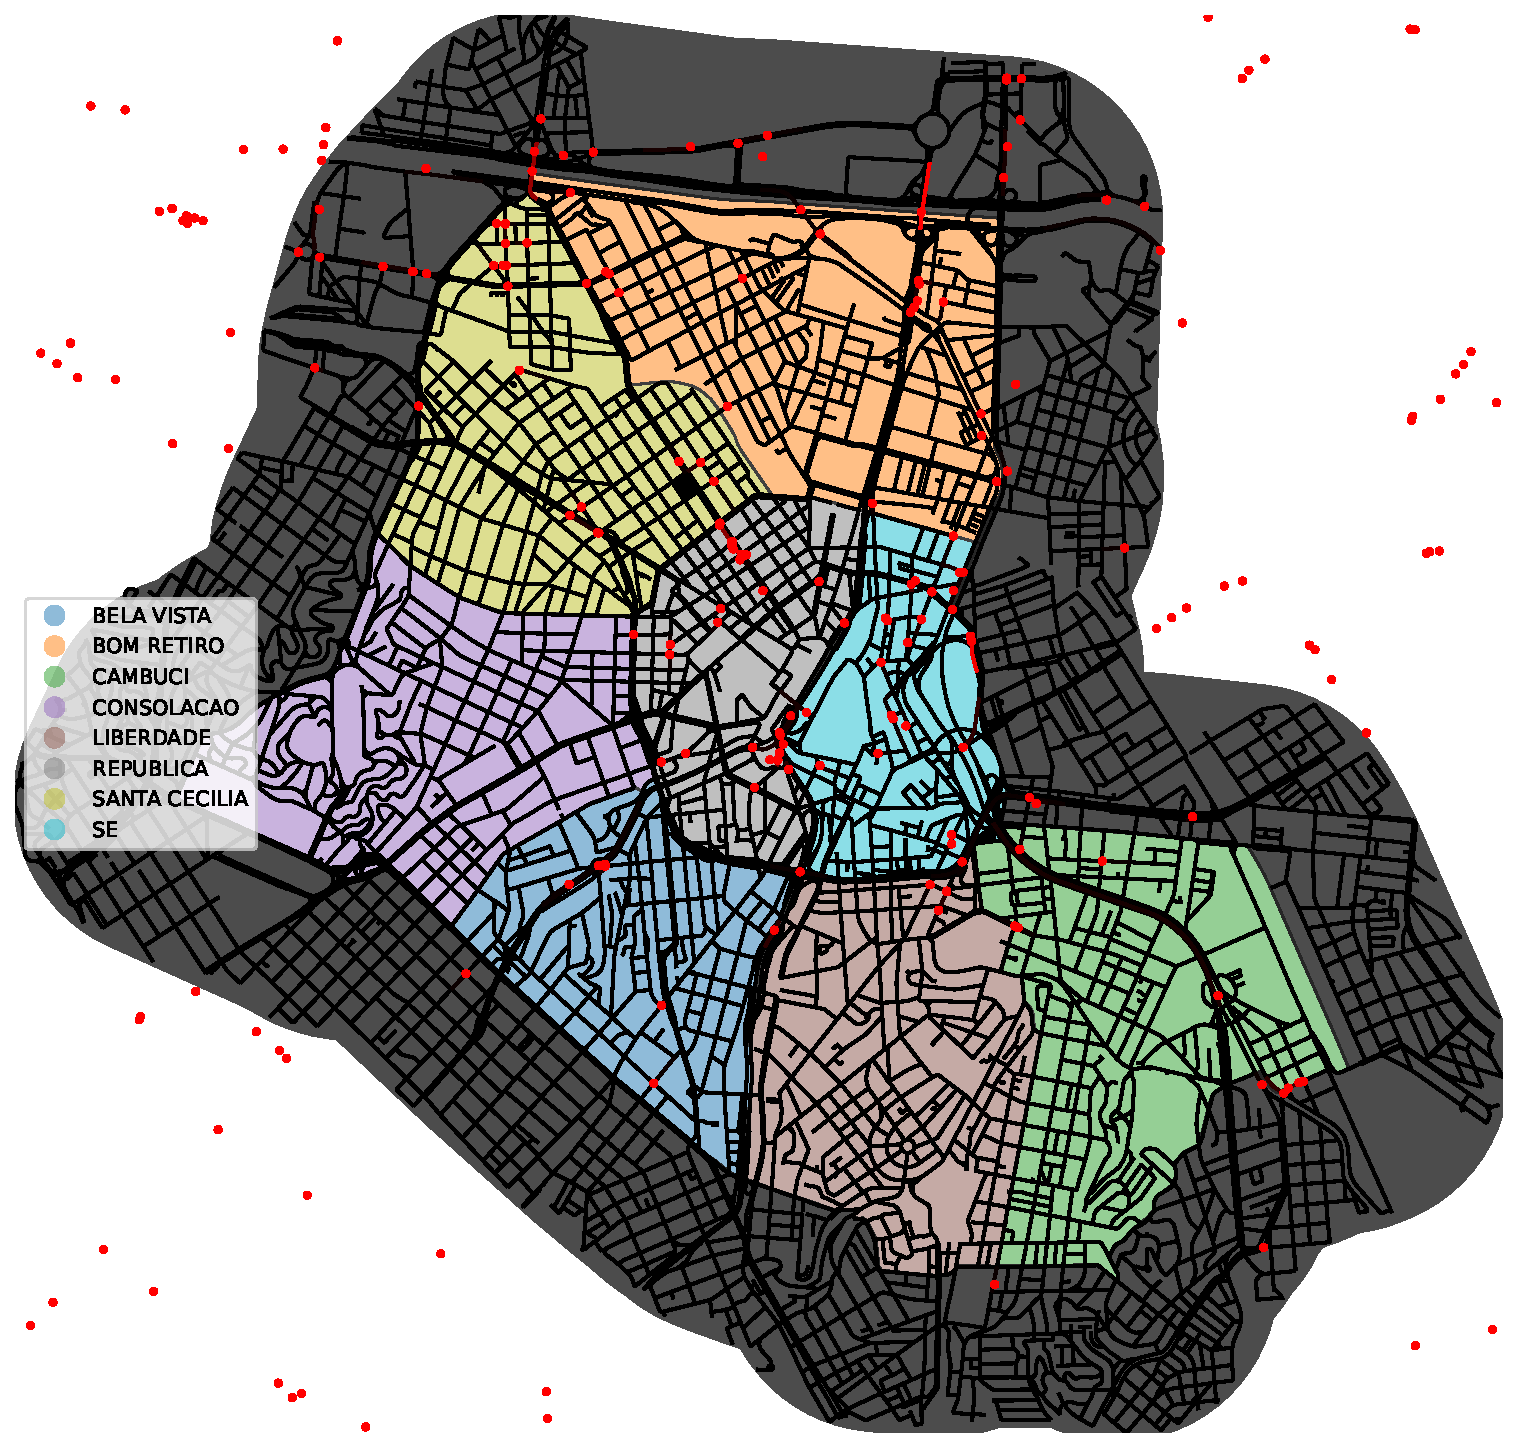
\includegraphics[width=0.8\columnwidth]{figures/floods_center.pdf}
    \caption{Study area (central São Paulo), showing the 2019 flood occurrences and the street network.}
    \label{fig:studyarea}
\end{figure}

The resulting graph has $8,714$ streets and $5,637$ intersections, totaling 884 km of streets.
Each flood occurrence is matched to its nearest street in meters (UTM zone 23S, EPSG:31983) with a tolerance of 50 m. Of the 286 occurrences inside the study area, 282 were matched (98.6\%); the match rate is not sensitive to the tolerance (97.9\% at 25 m and 99.3\% at 100 m). This matching gives us 137 flooded streets (1.6\% of the network) concentrating 282 events.

Graphs are defined as $G = (V,E)$, in which $V$ is the set of vertices (or nodes), and $E$ is the set of edges (or links). Here, we use graphs to represent the street map, allowing us to compute graph metrics described in Table \ref{tab:metrics}. This representation is made by turning streets into nodes and their intersections into edges (the line graph of the street map). This way, we can look into the signatures flooded and non-flooded streets might have.


\begin{table}[H]
    \centering
    \caption{Description of each network metric used in this work. All metrics are computed at the street level.}
    \begin{tabularx}{\textwidth}{X|X}
         \hline
         \textbf{Metric} & \textbf{Description} \\
         \hline
         Degree & Number of connections of a node. \\
         \hline
         Mean Shortest Path & Mean shortest path length of all possible node combinations.\\
         \hline
         Closeness & The inverse of the mean distance from a node to all others; how close the street is to the rest of the network.\\
         \hline
         Betweenness & The importance of a node in the network's shortest paths. It accounts for the number of shortest paths that go through the node.\\
         \hline
         Subgraph centrality \cite{Estrada2008} & The participation of a node in all closed walks starting and ending on it, a generalization of the concept of communicability.\\
         \hline
         PageRank \cite{page1999} & The stationary probability of a random walker visiting the node.\\
         \hline
         Vulnerability \cite{Latora2004, Goldshtein2004} & Metric to spot the critical components of a critical infrastructure network. For each street $s$, $V(s) = (E - E_{-s})/E$, where $E$ is the global efficiency \cite{Latora2001} of the network and $E_{-s}$ the efficiency without the street.
         \\
         \hline
    \end{tabularx}

    \label{tab:metrics}
\end{table}

We also computed the eigenvector centrality, but we excluded it from the analysis: it localizes on the densest cluster of the network, leaving a median of zero on both flooded and non-flooded streets, its ranking is unstable to the network boundary, and it carries no signal after the terrain controls. Elevation and absolute grade enter the analysis side by side with the topological metrics.

The corresponding source code, the executed notebooks, and all derived datasets are available at the GitHub repository given in the data availability statement.

\subsection{Mann-Whitney U Test}

The Mann-Whitney U Test is a non-parametric test for comparing two populations, $X$ and $Y$.
In particular, using two random (iid) samples from $X$ and $Y$, we want to test the null hypothesis that the probability of $X$ being greater than $Y$ is equal to the probability of $Y$ being greater than $X$.

Consider $\boldsymbol{X} = (X_1, X_2, \ldots, X_{n_1})$ and $\boldsymbol{Y} = (Y_1, Y_2, \ldots, Y_{n_2})$ as random samples from $X$ and $Y$ respectively.
The test works by merging the $\boldsymbol{X}$ and $\boldsymbol{Y}$ and ranking their values from smallest to largest.
Then the sample is split again, but now with their ordering values instead.

We compute the statistics $U_1$ and $U_2$ from their ranks as follows:
\begin{equation}
U_1 = n_1 n_2  + \frac{n_1(n_1+1)}{2} - R_1,
\end{equation}
and
\begin{equation}
    U_2 = n_2 n_1  + \frac{n_2(n_2+1)}{2} - R_2,
\end{equation}
where $n_1$ is the number of values of the first sample and $n_2$ of the second sample. $R_1$ and $R_2$ are each sample's sum of ranks.
The null hypothesis here is that $R_1$ and $R_2$ are equal.

We use the statistic $U = U_1$ of the first sample (flooded streets), whose expected value is
\begin{equation}
    \mu_U = \frac{n_1n_2}{2},
\end{equation}
and its standard error, with the correction for ties,
\begin{equation}
    \sigma_U = \sqrt{\frac{n_1n_2(n_1+n_2+1)}{12}},
\end{equation}
which allows us to compute the z-value
\begin{equation}
    z = \frac{U - \mu_U}{\sigma_U}.
\end{equation}

This z-value can then be compared to its distribution under the null hypothesis (standard normal), yielding a p-value. Since we test several metrics simultaneously, we correct the p-values for multiple comparisons with the Benjamini-Hochberg procedure \cite{benjamini1995}, and we reject the null hypothesis at a significance level of 0.5\% (or 0.005).
Together with each p-value we report the rank-biserial correlation $r = 2U/(n_1 n_2) - 1$ as effect size: $r > 0$ means the flooded streets have higher values of the metric.

To provide a concise overview of our methodology, we partition the dataset into two categories: flooded and non-flooded streets. Subsequently, we employed violin plots as visual tools for analyzing and visualizing the distributions within each category, and the Mann-Whitney U test to assess whether the metrics calculated for flooded streets exhibited any discernible signatures.

Streets are not independent observations: flooded streets cluster along drainage lines. We quantify this clustering with Moran's I on the flood indicator, and we address it with three analyses that take the structure into account. First, logistic regression models of the flooded/non-flooded label on each centrality (one at a time, standardized), controlling for elevation, absolute grade, street length, number of lanes, and highway class, together with Poisson and negative binomial models on the number of events per street with the street length as exposure offset. Second, a predictive model (random forest and gradient boosting) evaluated with spatial cross-validation, where the folds are blocked by district, so no model is evaluated on a district it has seen. Third, a resilience simulation, removing the flooded streets from the graph and measuring the degradation of the network efficiency against random and betweenness-targeted removals of the same size.

\subsection{Does the signature generalize? A city-wide district analysis}
\label{sec:districts}

The central claim of this work is that central streets flood more. The analyses above test it on one study area; however well it holds there, it is still one observation. The purpose of the district analysis is to make the claim stronger by showing that the pattern repeats in many areas: we repeat the flooded versus non-flooded comparison independently in every district of São Paulo with at least 5 flood events in 2019 (52 of the 96 districts, concentrating 1,114 of the 1,165 events), each district with its own street graph from OSM, its own metrics, and its own flood matching, so each one is an independent replication of the claim. Only streets whose midpoint falls inside the district enter its test. The per-district effect sizes are then pooled with a DerSimonian-Laird random-effects meta-analysis \cite{dersimonian1986}, which also quantifies the heterogeneity of the effect across the city ($I^2$).

We also compare two modeling designs on the districts shared by both: computing the metrics on the whole central network and splitting the streets by district (Design 1), against computing the metrics on each district's own graph (Design 2). Agreement between the designs means the signature is robust to this modeling choice.

The decomposition also gives every street a \emph{local} rank inside its own district's network, and we exploit it in three street-level views: the percentile of each flooded street within its own district's ranking (pooled over all districts against the uniform null), the comparison of the local rank against the global rank in the central districts, and an extended meta-regression asking whether the district character -- terrain relief, street-orientation entropy, circuity, and distance to the Tietê and Pinheiros rivers -- explains where the effect is strong.

\subsubsection{Buffer sensitivity}
\label{sec:buffer}

Cutting a graph at the district border creates artificial dead-ends: border streets lose degree, closeness, and betweenness \cite{gil2017}. A buffer restores each in-district street's neighborhood, but the buffer size should be chosen empirically, not guessed. For three districts of different sizes (Sé, Vila Matilde, and Cidade Ademar) we build the graph with buffers of 0, 250, 500, and 1000 m and check, against the 1000 m reference, the Spearman correlation of each metric's ranking and the shift in the closeness effect size. With no buffer the closeness effect can even flip sign (Vila Matilde: $-0.22$ against $+0.66$ of the reference); at 500 m the closeness ranking still correlates only 0.947 with the reference and the effect size shifts up to 0.145. No smaller buffer met our criteria (all rank correlations $\geq 0.99$ and effect shift $\leq 0.02$), so we adopt the 1000 m buffer everywhere.

\section{Results and discussion}
\label{ch:chap3}

We illustrate our results using violin plots, tables, forest plots, and maps. The violin plots help to visualize the differences in the separated datasets, one with flooded and the other with non-flooded streets; the tables and the odds-ratio plot depict the results from the Mann-Whitney U test and the regression models; the forest plots and the maps show how the effect distributes across the city.

\subsection{Flooded versus non-flooded streets}

Figure \ref{fig:todos_violin} shows the violin plots of each metric, comparing the statistics side by side. The differences are apparent in the mean shortest path length, closeness, betweenness, and vulnerability panels, and also in the elevation: flooded streets sit lower (median 732 m against 752.5 m) and are flatter.

\begin{figure}[H]
    \centering
    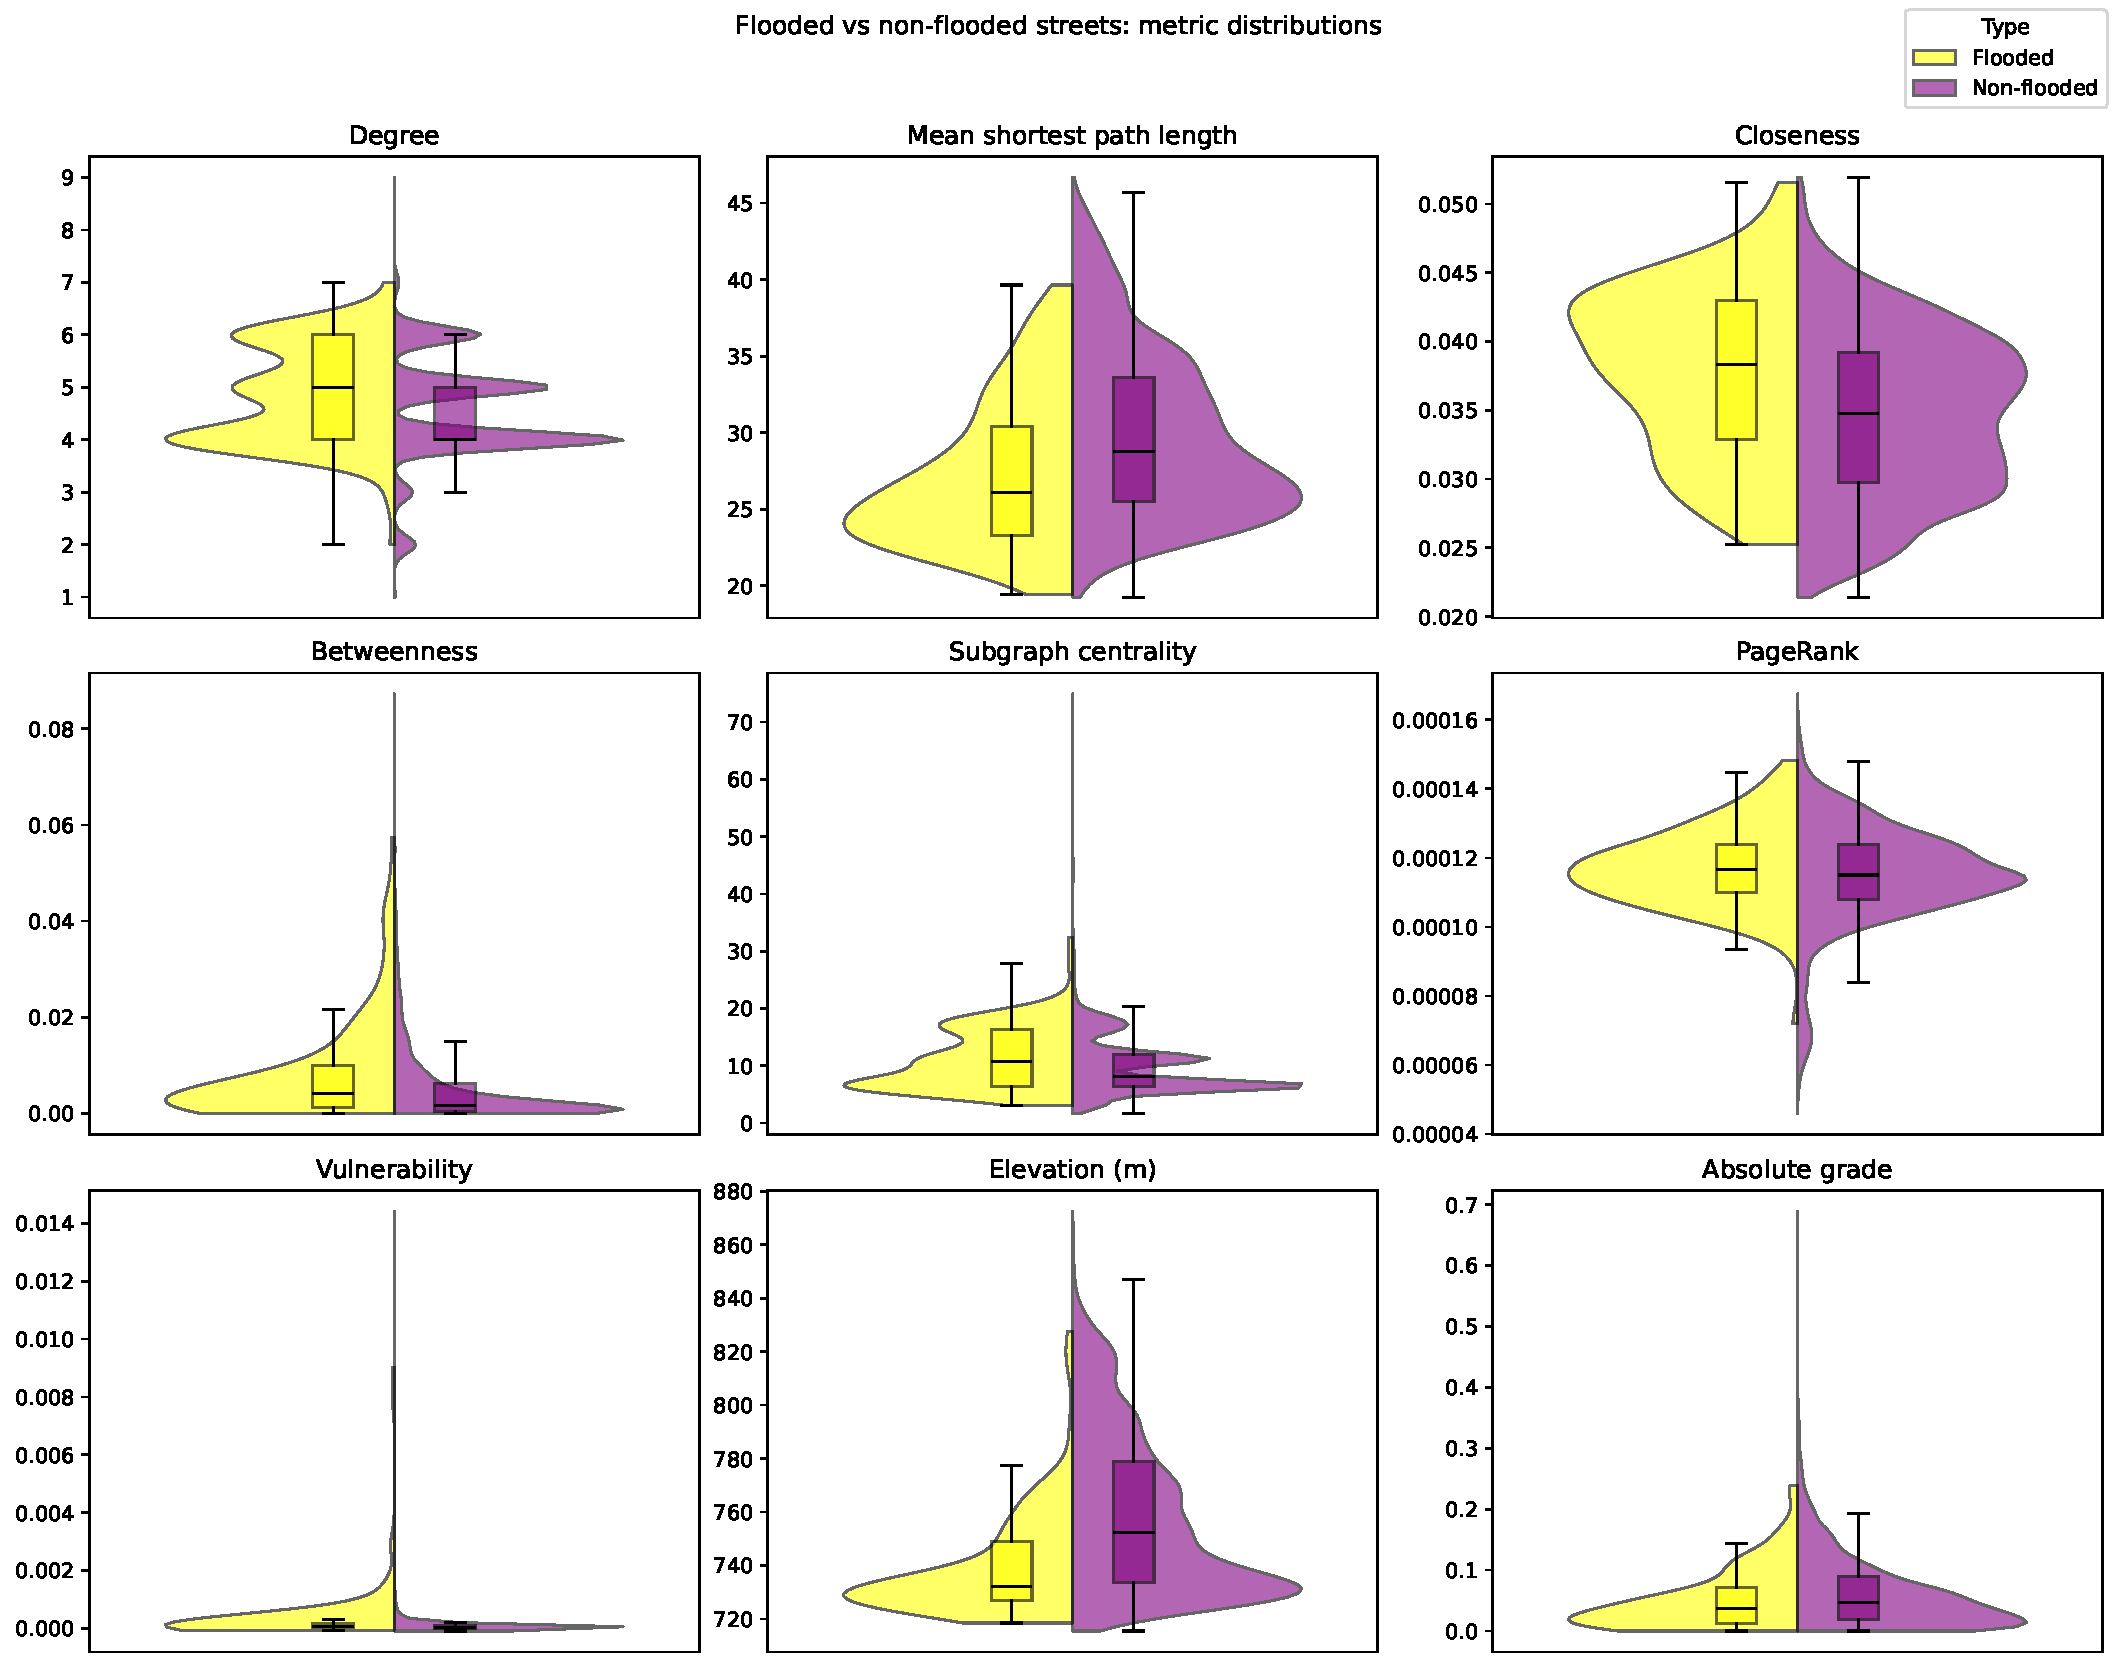
\includegraphics[width=\textwidth]{figures/violins_all_metrics.pdf}
    \caption{Series of violin plots, where yellow (left side) represents the flooded streets, while purple (right side) represents non-flooded streets, with a box plot inside. The panels are the seven network metrics plus elevation and absolute grade.}
    \label{fig:todos_violin}
\end{figure}

To mathematically compare distributions pairwise, we apply the Mann-Whitney U test (Table \ref{tbl:mwu}), reporting the rank-biserial correlation as effect size and the Benjamini-Hochberg corrected p-values.

\begin{table}[H]
\centering
\caption{Medians, rank-biserial correlations ($r > 0$: flooded streets have higher values), and corrected p-values comparing flooded ($n_1 = 137$) and non-flooded ($n_2 = 8,577$) streets. Highlighted in blue are the metrics with a corrected p-value under 0.005.}\label{tbl:mwu}
\begin{tabular}{l|cc|cc}
\toprule
Metric & Median flooded & Median non-flooded & $r$ & p-value (BH) \\
\midrule
\rowcolor{LightCyan}
Vulnerability & $1.0\times10^{-4}$ & $2.9\times10^{-5}$ & $+0.343$ & $<10^{-4}$ \\
\rowcolor{LightCyan}
Mean shortest path & 26.11 & 28.79 & $-0.286$ & $<10^{-4}$ \\
\rowcolor{LightCyan}
Closeness & 0.0383 & 0.0347 & $+0.286$ & $<10^{-4}$ \\
\rowcolor{LightCyan}
Betweenness & 0.0042 & 0.0017 & $+0.265$ & $<10^{-4}$ \\
\rowcolor{LightCyan}
Degree & 5 & 4 & $+0.161$ & $9\times10^{-4}$ \\
Subgraph centrality & 10.71 & 8.06 & $+0.115$ & $0.025$ \\
PageRank & $1\times10^{-4}$ & $1\times10^{-4}$ & $+0.069$ & $0.164$ \\
\midrule
\rowcolor{LightCyan}
Elevation (m) & 732.0 & 752.5 & $-0.430$ & $<10^{-4}$ \\
Absolute grade & 0.037 & 0.047 & $-0.114$ & $0.025$ \\
\botrule
\end{tabular}
\end{table}

We reject the null hypothesis for five of the seven network metrics. The vulnerability presents the largest effect among the topological metrics, and the mean shortest path and closeness follow (they carry the same ranking, one being a monotone function of the other). It is crucial to notice that the largest effect of all belongs to the elevation: floods are, before anything else, a phenomenon of the low streets. This is exactly why the next subsection controls for it.

Before that, one caveat. Flooded streets cluster along drainage lines, so the streets are not independent observations and the p-values above are optimistic. Moran's I on the flood indicator confirms the clustering ($I = 0.067$, $p = 0.001$). The regressions and the spatially blocked cross-validation below are the analyses that take this structure into account.

\subsection{Controlling for terrain}

The central question for this work: do the network metrics predict flooding \emph{after} controlling for terrain? São Paulo's arterial avenues often run along valley bottoms (\textit{fundo de vale}), so centrality could be a proxy for elevation. We fit one logistic model per centrality (standardized), always controlling for elevation, absolute grade, street length, number of lanes, and highway class. Figure \ref{fig:oddsratios} shows the odds ratios.

\begin{figure}[H]
    \centering
    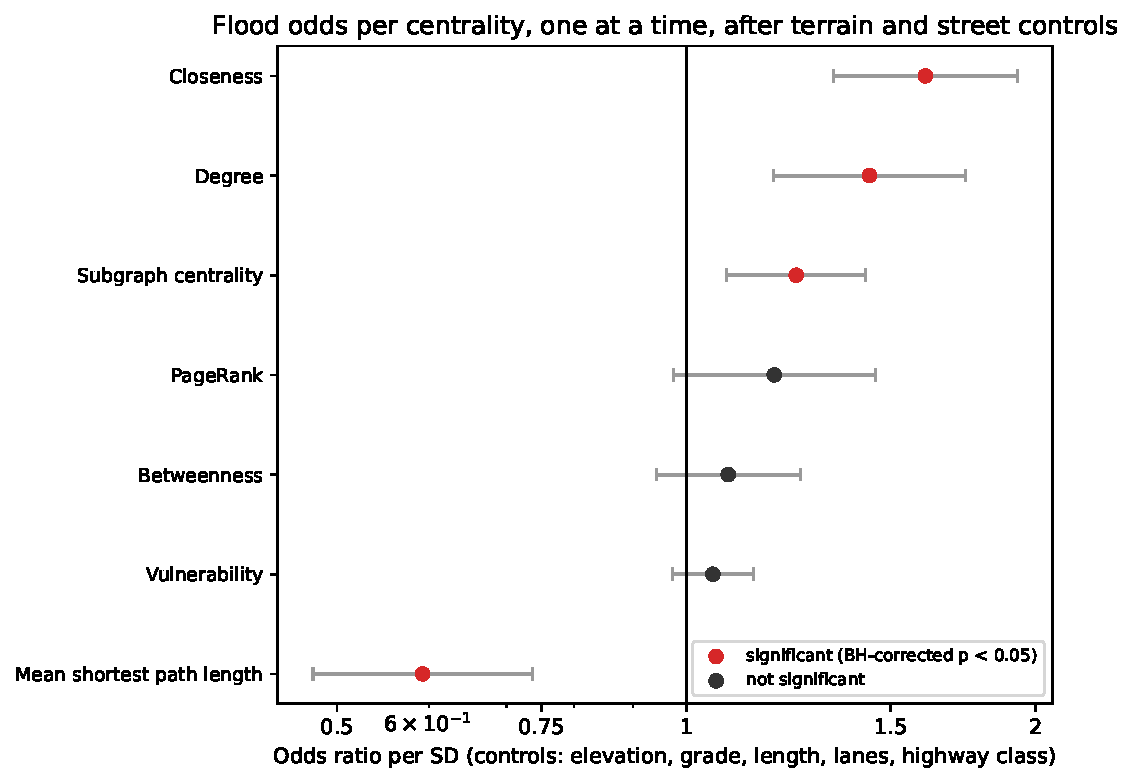
\includegraphics[width=0.8\columnwidth]{figures/logit_odds_ratios.pdf}
    \caption{Odds ratio of flooding per standard deviation of each metric, one model at a time, controlling for elevation, grade, length, lanes, and highway class. Values above 1 increase the flood odds; red markers are significant after correction.}
    \label{fig:oddsratios}
\end{figure}

Closeness (odds ratio 1.61 per standard deviation, CI 95\% [1.34, 1.93]), mean shortest path (0.59, [0.48, 0.74]), degree (1.44, [1.19, 1.74]), and subgraph centrality (1.24, [1.08, 1.43]) remain significant after the controls. Betweenness (1.09), PageRank (1.19), and vulnerability (1.05) do not. The elevation stays the strongest single predictor in every model (odds ratio $\approx 0.4$ per standard deviation).

The vulnerability case deserves a comment. Its univariate effect is the largest of all topological metrics, and it is not a terrain proxy: its Spearman correlation with elevation is essentially zero (0.006). What absorbs it in the regression are the street attributes -- highway class and lanes -- since the vulnerable streets are largely the major corridors. Its distribution is also extremely skewed (the most vulnerable street weighs around 500 times the median one), which weakens a linear per-standard-deviation term. The accurate statement is that floods concentrate on the corridors whose loss costs the network the most, not that vulnerability carries a signal independent of what the street already is.

The count models on the number of events per street (Poisson and negative binomial, with the street length as exposure offset) tell the same story: elevation dominates (rate ratio 0.32 per standard deviation), the highway classes multiply the event rate by 7 to 15 times against the reference class, and among the centralities only the degree remains (rate ratio 2.6, $p = 0.051$ Poisson, $p = 0.026$ negative binomial).

\subsection{The pattern repeats across the city}

This is where the main claim gains its strength. One study area showing that central streets flood more is one observation; here the same comparison runs independently in every testable district, and the pattern repeats. Figure \ref{fig:forest_bet} presents the forest plot of the betweenness effect in the 42 testable districts: the effect is positive in \textbf{every single district}, with no measurable heterogeneity (pooled $r = +0.30$ [0.25, 0.35], $I^2 = 0\%$). The closeness presents the largest pooled effect ($r = +0.34$ [0.26, 0.42], positive in 36 of 42 districts) but varies in strength across the city ($I^2 = 56\%$); the degree ($+0.14$) and PageRank ($+0.12$) are smaller and homogeneous.

\begin{figure}[H]
    \centering
    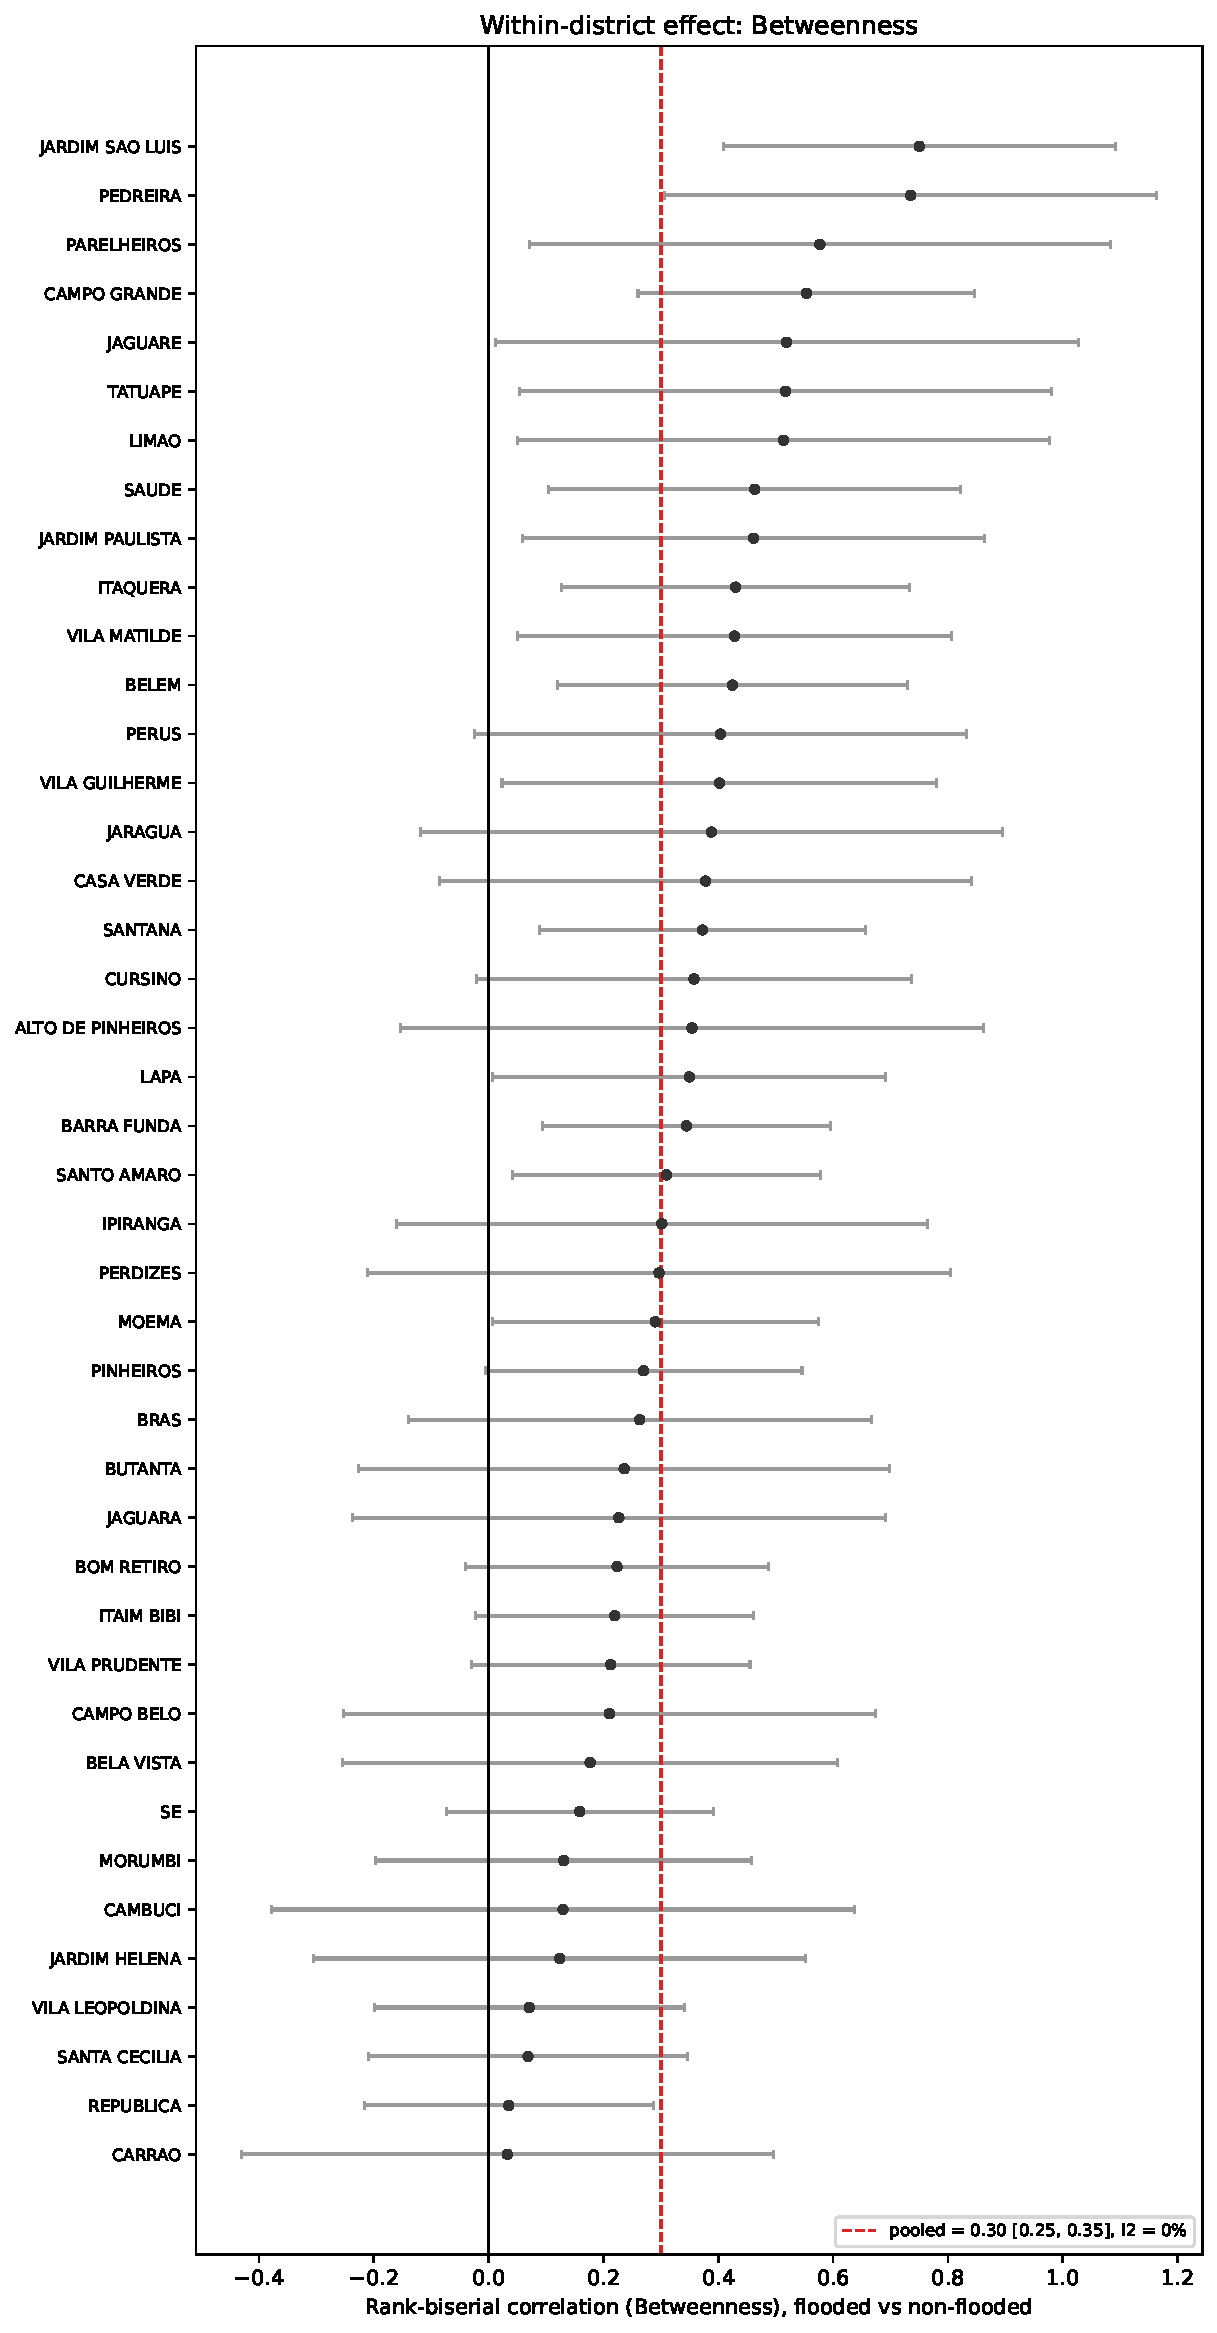
\includegraphics[width=0.85\columnwidth]{figures/forest_betweenness.pdf}
    \caption{Within-district effect size of the betweenness (rank-biserial correlation with 95\% CI), one row per district. The effect is positive in all 42 districts, with $I^2 = 0\%$.}
    \label{fig:forest_bet}
\end{figure}

The district decomposition gives every street a rank inside its own district's network, and this local view makes the generalization concrete. Figure \ref{fig:local_pct} pools, over all districts, the percentile of each flooded street within its own district's ranking: under the null the percentiles would be uniform, and instead \textbf{the median flooded street is more central than 75\% of the streets of its own district} by closeness (Wilcoxon against the uniform, $p = 1.7\times10^{-29}$), 70\% by betweenness, and 60\% by degree. This is a street-level statement: the signature is not the center of the city being central, it repeats inside each neighborhood.

\begin{figure}[H]
    \centering
    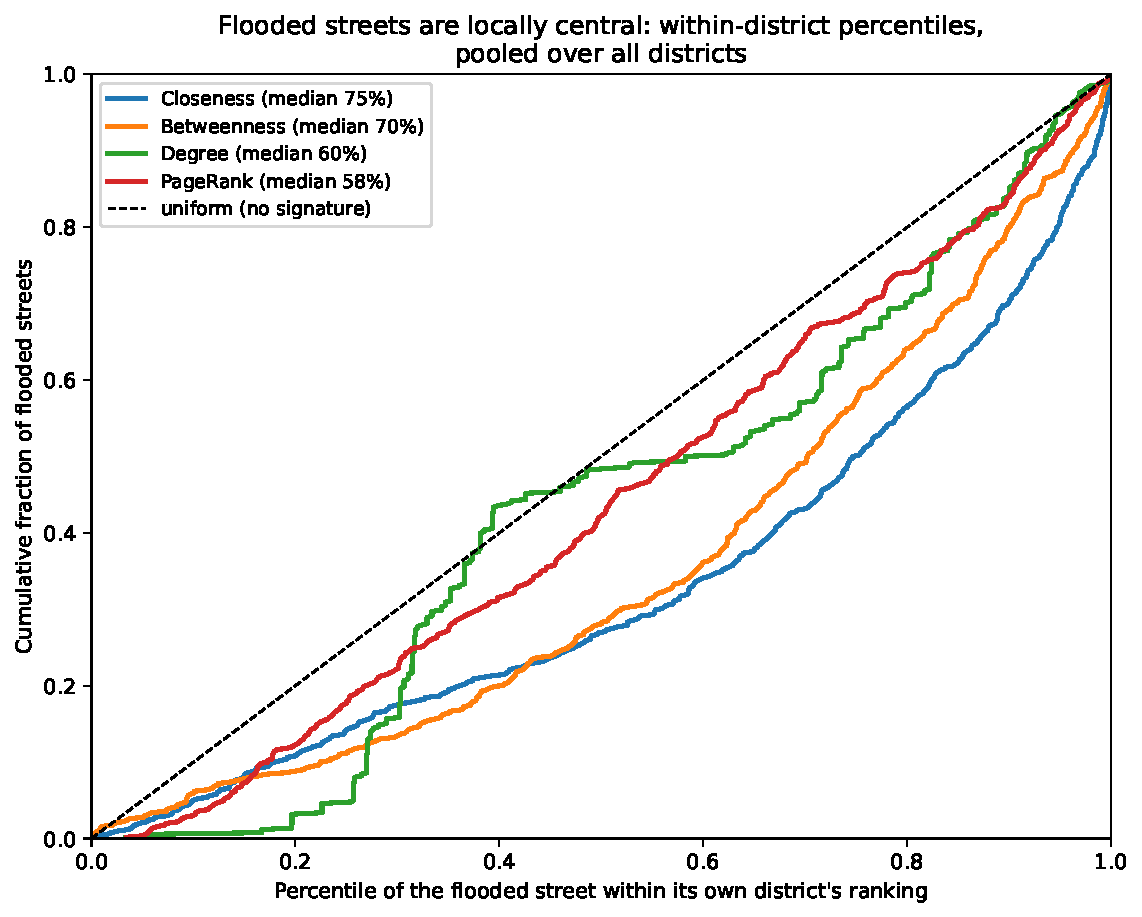
\includegraphics[width=0.75\columnwidth]{figures/local_percentiles.pdf}
    \caption{Cumulative distribution of the within-district percentile of the flooded streets, pooled over all districts, one curve per metric. The dashed diagonal is the uniform null (no signature).}
    \label{fig:local_pct}
\end{figure}

Figure \ref{fig:multiples} shows nine districts spanning the effect range, each drawn with its own network and colored by its own local closeness percentile. In the strong-effect districts the flood events visibly follow the district's central spine. The weak and negative districts are also informative: in Santana and Casa Verde the floods line the southern edge of the district -- the Tietê floodplain -- where the locally peripheral streets are precisely the low ones, so terrain overrides topology.

\begin{figure}[H]
    \centering
    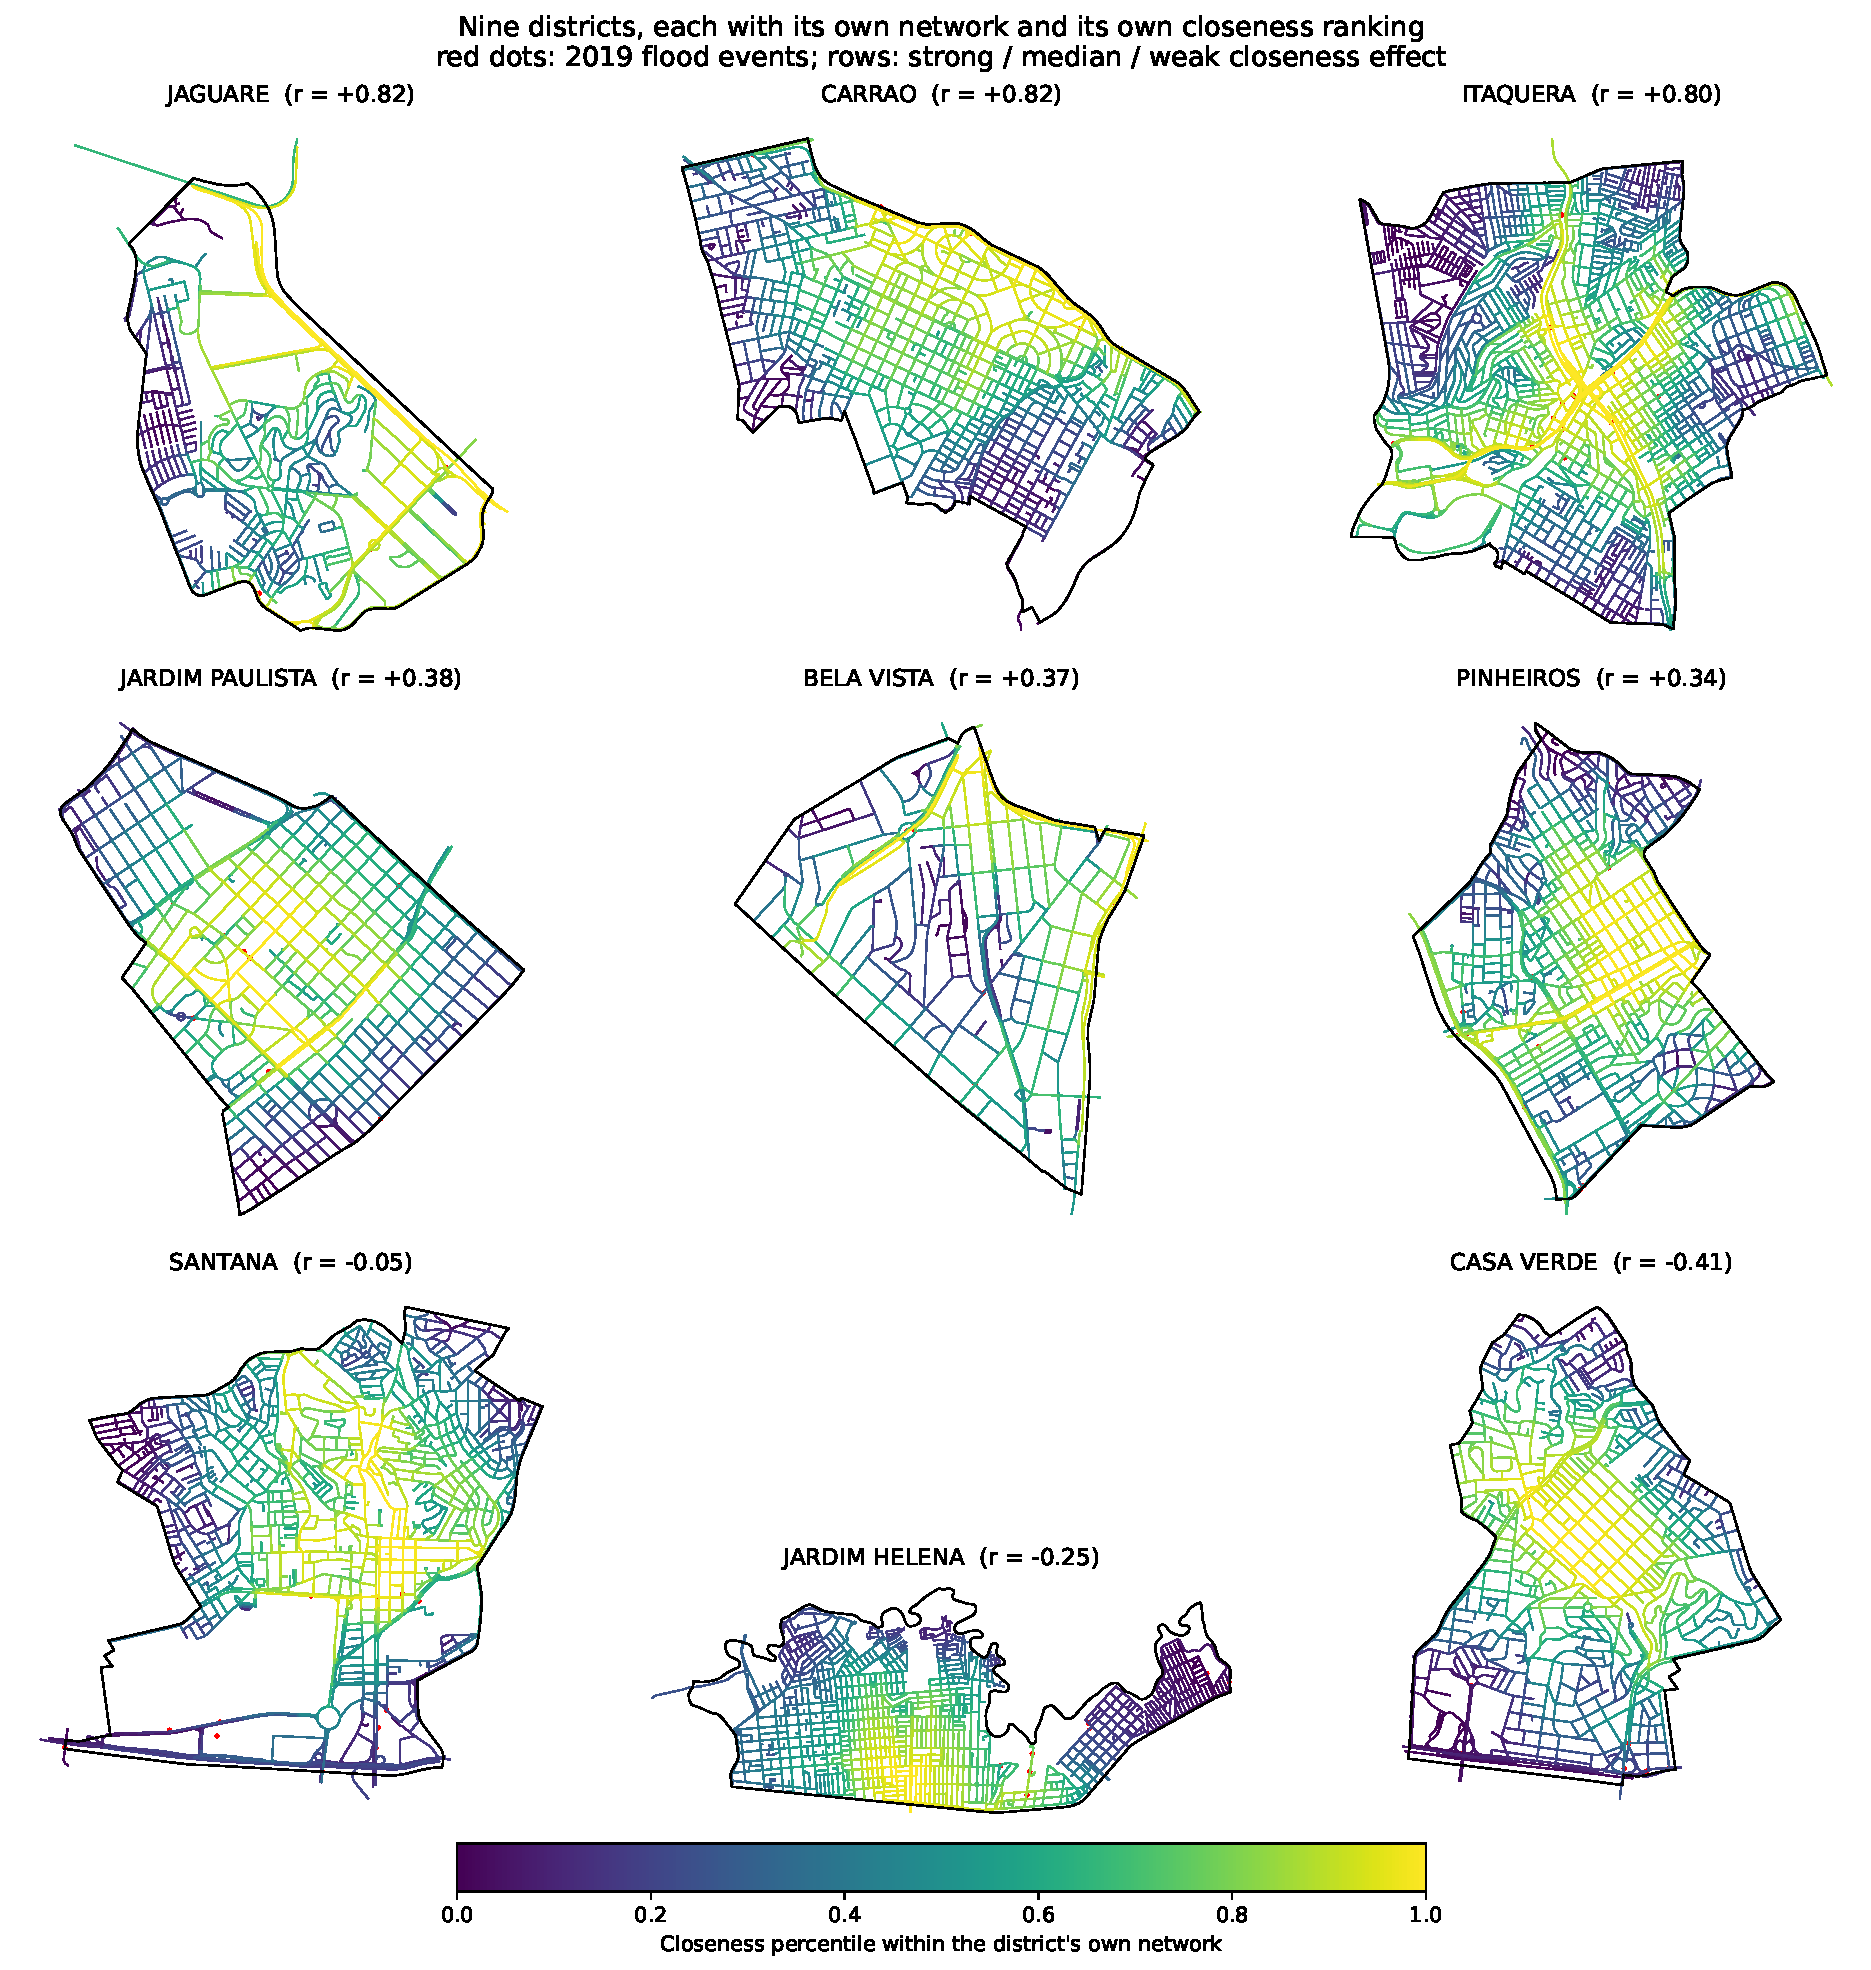
\includegraphics[width=\textwidth]{figures/district_small_multiples.pdf}
    \caption{Nine districts, each with its own network colored by its own closeness percentile (yellow: locally central), spanning strong (top), median (middle), and weak or negative (bottom) closeness effects. Red dots are the 2019 flood events.}
    \label{fig:multiples}
\end{figure}

Being central for the district and being central for the city are different things, and the flooded streets are central in both readings -- the claim holds at the two scales. For the seven central districts covered by both networks, Figure \ref{fig:localglobal} compares each street's closeness percentile within its own district (local rank) against its percentile within the whole central network (global rank): the two rankings only partially agree ($\rho = 0.53$), yet the flooded streets sit high in both (median 81\% globally, 68\% locally). A visible group of flooded streets is globally central but locally peripheral -- through-corridors that cross quieter districts -- which carries its own planning implication: those are city-scale arterials, not neighborhood bottlenecks, and their flooding is a problem for the whole city, not only for the district they cross.

\begin{figure}[H]
    \centering
    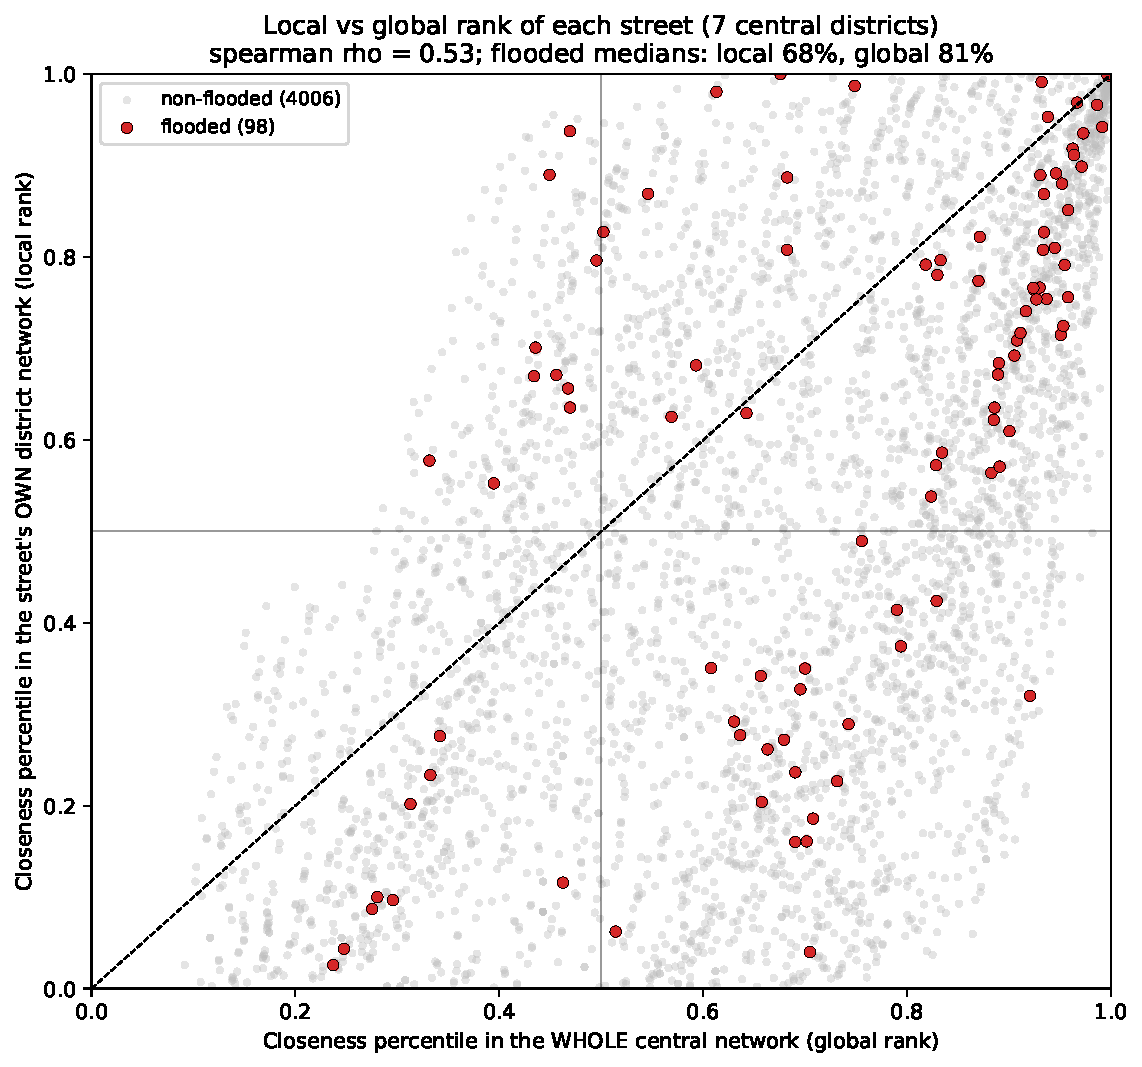
\includegraphics[width=0.75\columnwidth]{figures/local_vs_global_rank.pdf}
    \caption{Local rank (closeness percentile within the street's own district network) against global rank (percentile within the whole central network) for the seven central districts. Flooded streets in red.}
    \label{fig:localglobal}
\end{figure}

Figure \ref{fig:choropleth} maps the closeness effect on the district polygons. Within the central area, a fixed-effects test also detects that the closeness effect differs in strength across the central districts (likelihood-ratio test of the interaction, $p = 0.007$), consistent with the moderate $I^2$: the signature varies in intensity, rarely in direction. We then ask what explains where the effect is strong, with a meta-regression on the district character: mean elevation, terrain relief (elevation standard deviation), street-orientation entropy, circuity, distance to the Tietê and Pinheiros rivers, and network size. None of them does ($R^2 = 0.02$, $F$-test $p = 0.99$). The variation in strength is presumably governed by the local drainage infrastructure, which we do not observe.

\begin{figure}[H]
    \centering
    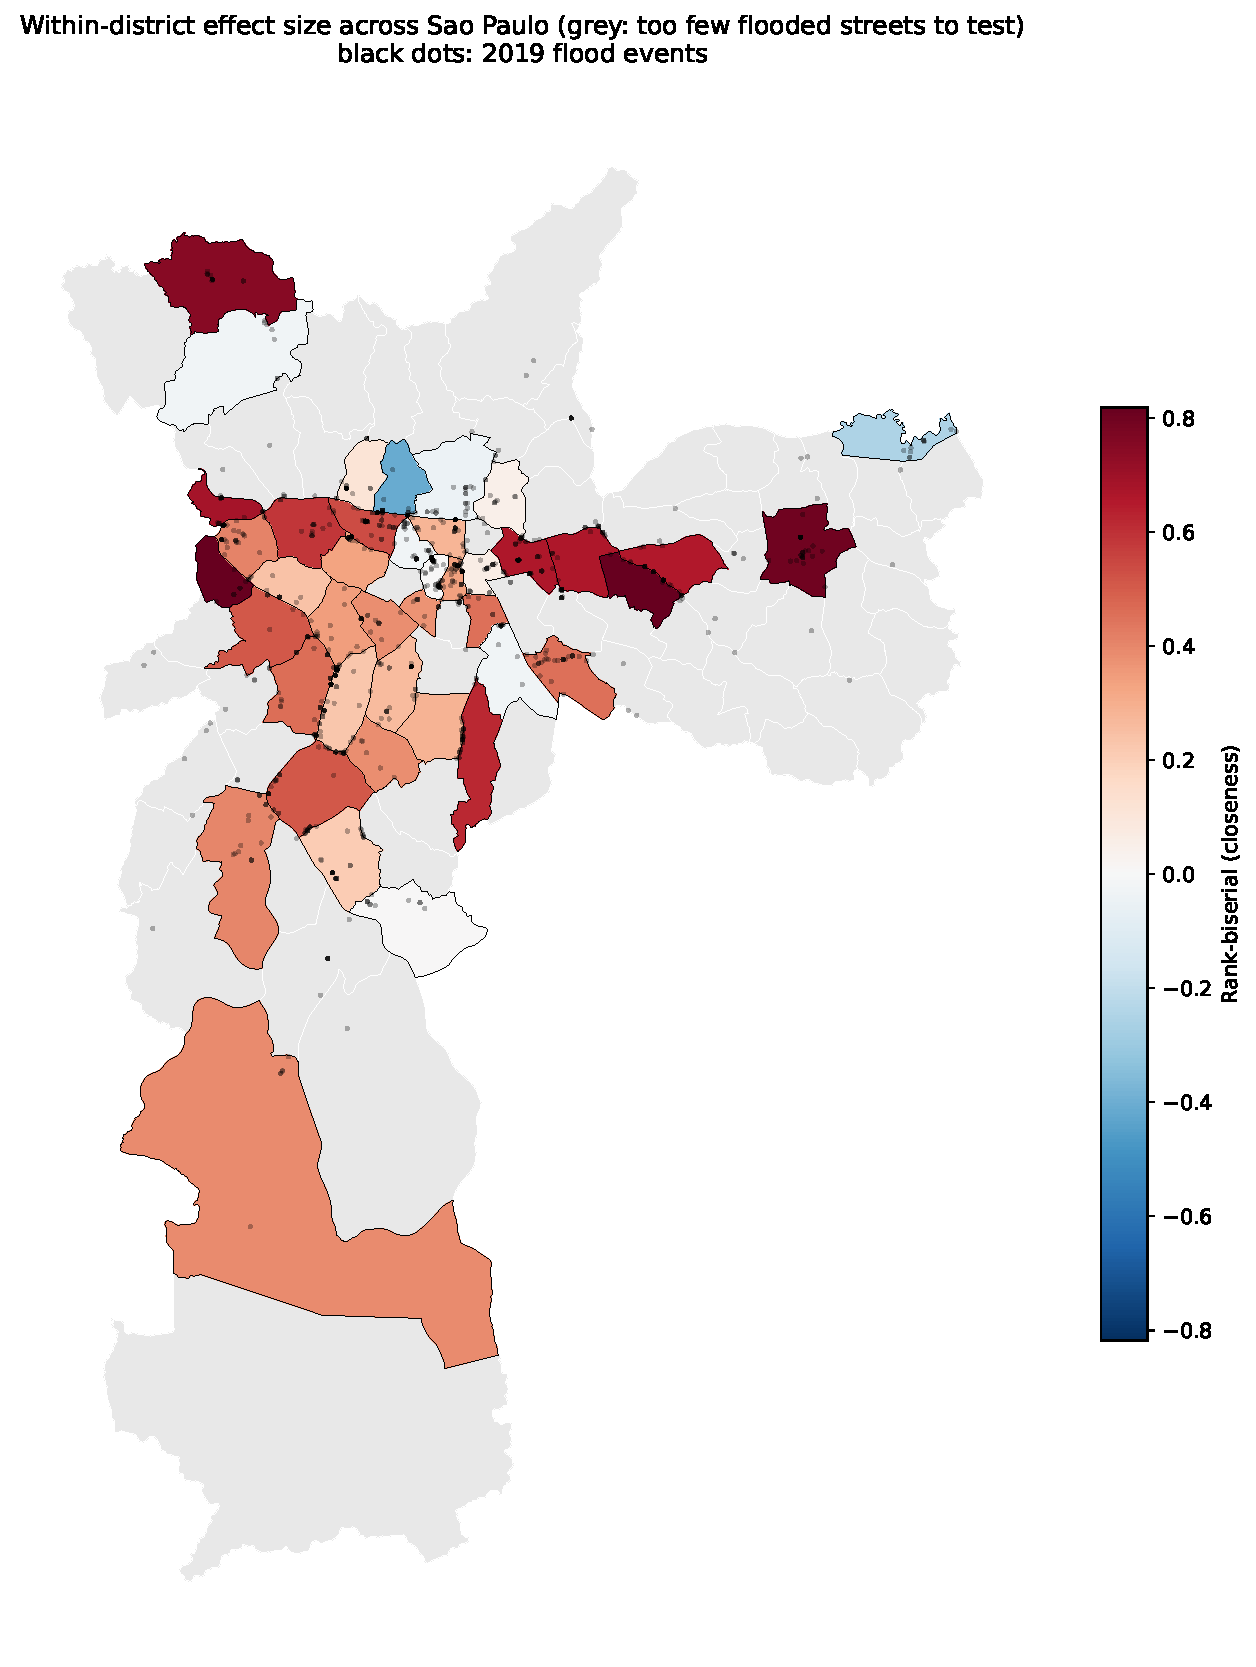
\includegraphics[width=0.85\columnwidth]{figures/district_effect_map.pdf}
    \caption{Within-district closeness effect size across São Paulo. Grey districts have too few flooded streets to test; black dots are the 2019 flood occurrences.}
    \label{fig:choropleth}
\end{figure}

Finally, we compare the two designs on the 40 district-metric pairs shared by both: the effect sizes correlate ($\rho = 0.56$, $p = 1.7\times10^{-4}$) and agree in sign in 92\% of the pairs (Figure \ref{fig:designs}). The signature does not depend on whether a street's metrics see the whole central network or only its own district.

\begin{figure}[H]
    \centering
    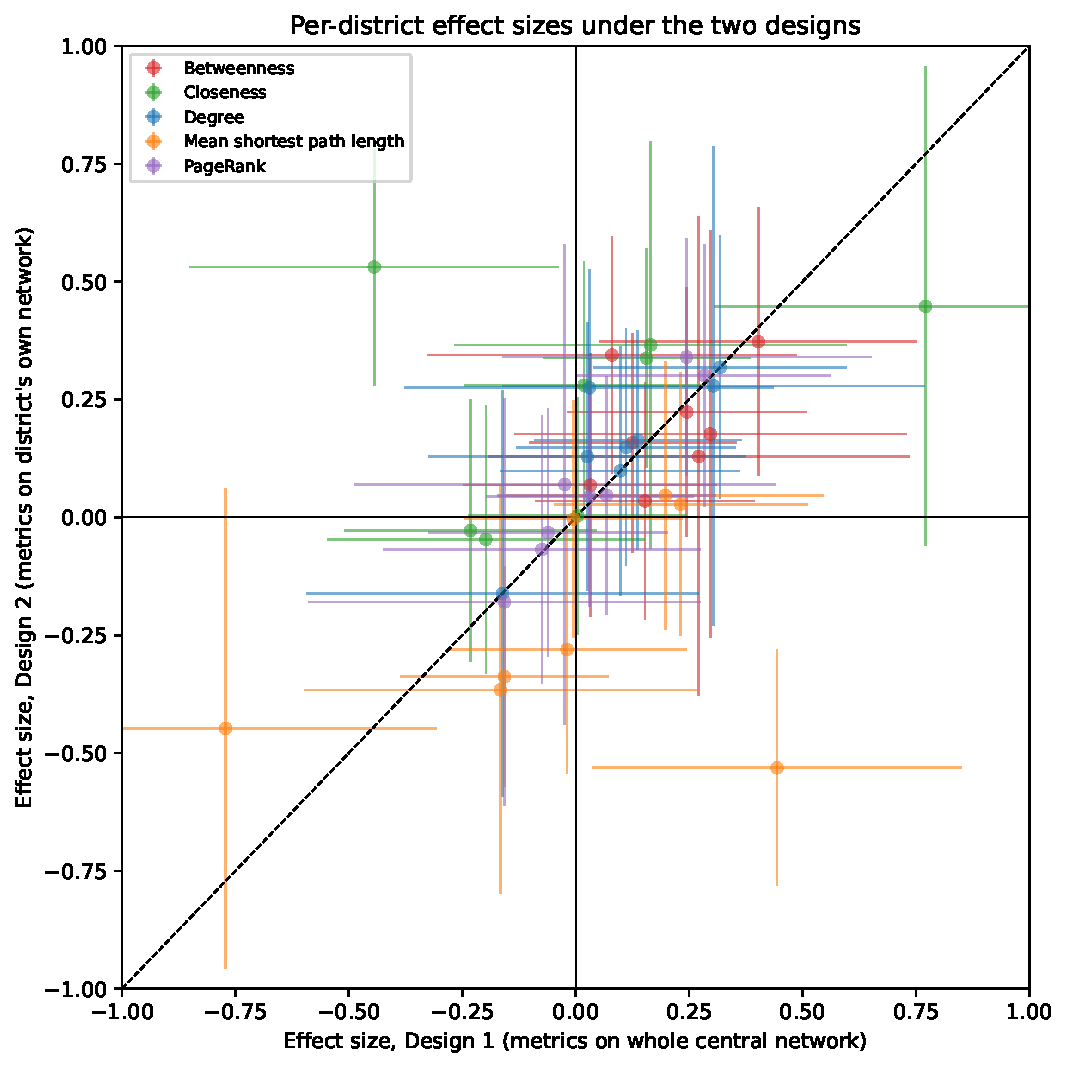
\includegraphics[width=0.7\columnwidth]{figures/design_comparison.pdf}
    \caption{Per-district effect sizes under the two designs: metrics computed on the whole central network (horizontal) against metrics computed on the district's own network (vertical).}
    \label{fig:designs}
\end{figure}

\subsection{Impact: what do the floods do to the network?}

Now, we look into the impact side of the signature. Removing the 137 flooded streets from the graph (as during a storm where all flood points are active) cuts the network efficiency by 4.6\%, against $1.8\% \pm 0.65$ for removing 137 random streets ($z = 4.35$) and 2.0\% for removing the top-137 betweenness streets. Figure \ref{fig:resilience} shows the sequential removal curves. The floods hit the network harder than a targeted attack of the same size: the streets that flood are the ones the network can least afford to lose, which the per-street vulnerability already anticipated (Table \ref{tbl:mwu}).

\begin{figure}[H]
    \centering
    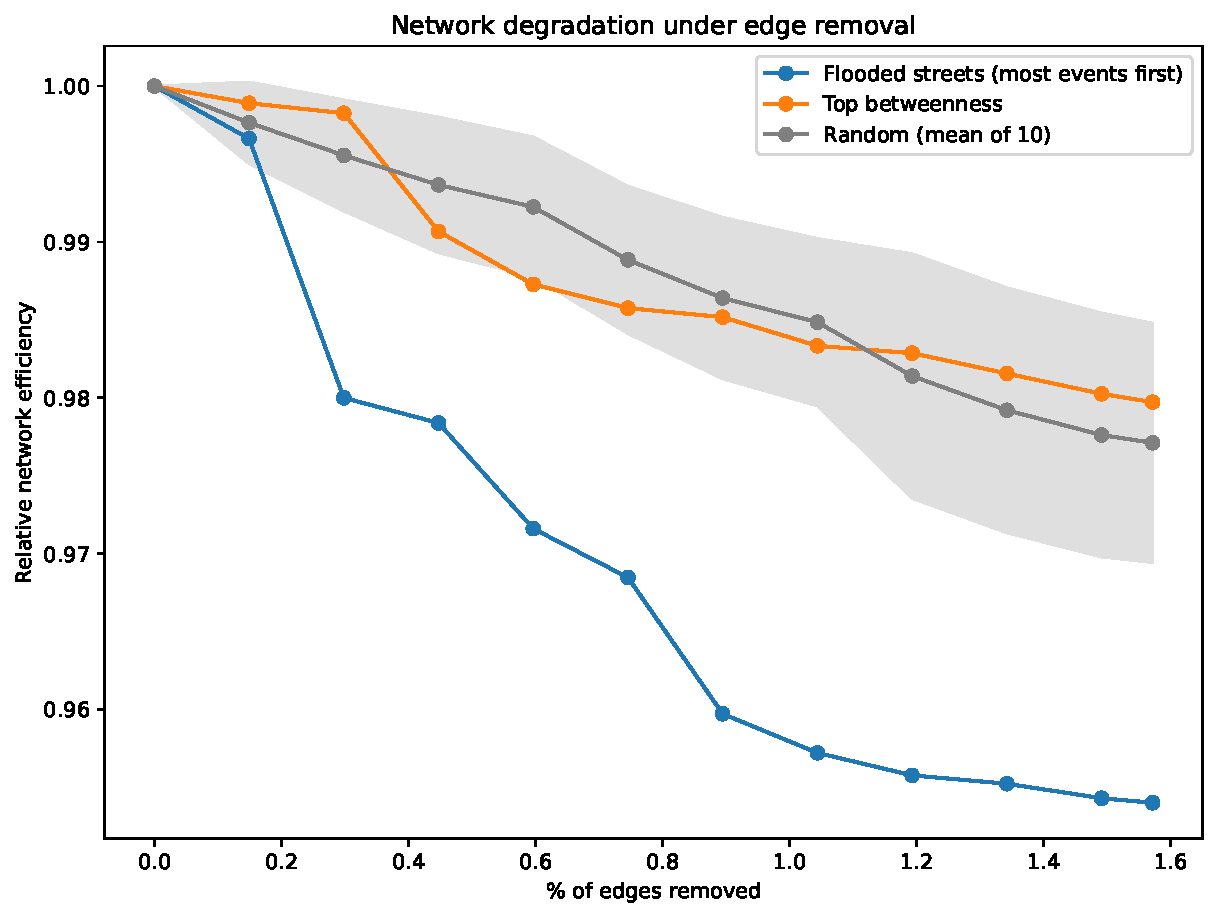
\includegraphics[width=0.75\columnwidth]{figures/resilience_curves.pdf}
    \caption{Network degradation under sequential removal: flooded streets (most events first), top betweenness, and random baseline.}
    \label{fig:resilience}
\end{figure}

\subsection{Recurrence}

Flooding is not evenly spread among the flooded streets: the recurrence is heavy-tailed, and the 10 most flooded streets concentrate 27\% of all matched events (Figure \ref{fig:recurrence}). We then ask whether the chronic repeat-flooders ($\geq 2$ events, $n = 43$) are topologically different from the one-time flooded streets ($n = 94$). They are not: no metric survives correction (all corrected $p \geq 0.64$). Network topology separates the streets that flood from the ones that do not, but among the streets that flood, it does not explain how often -- recurrence intensity is presumably governed by the local drainage. This negative result also argues against a reporting bias, where important streets would simply be reported more.

\begin{figure}[H]
    \centering
    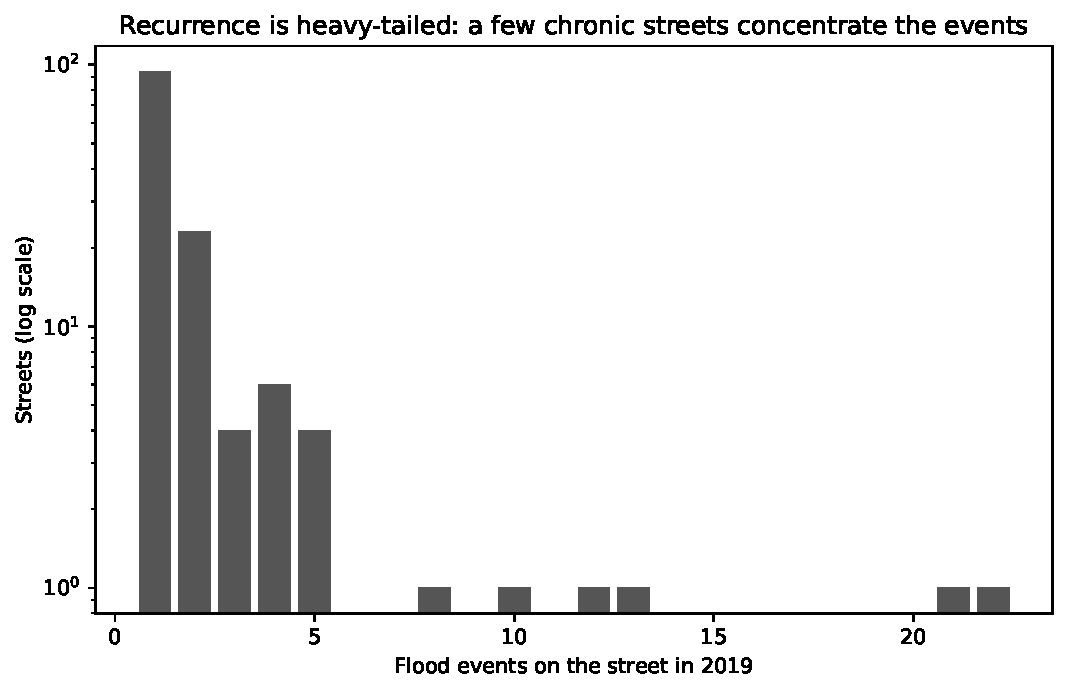
\includegraphics[width=0.7\columnwidth]{figures/recurrence_distribution.pdf}
    \caption{Recurrence of the flood events per street in 2019 (log scale). A few chronic streets concentrate the events.}
    \label{fig:recurrence}
\end{figure}

\subsection{Prediction and temporal robustness}

Can flood-prone streets be flagged from topology and terrain alone? With spatial cross-validation (folds blocked by district, so no model is evaluated on a district it trained on), a random forest reaches ROC-AUC of 0.74 and PR-AUC of 0.036 against a chance level of 0.016. Topology and terrain roughly double the precision of random targeting, but cannot pinpoint individual flood-prone streets; these are risk-screening covariates, not a forecasting tool. Figure \ref{fig:probmap} shows the cross-validated flood probability map, and the permutation importance points to the elevation and the mean shortest path as the features that matter out of district.

\begin{figure}[H]
    \centering
    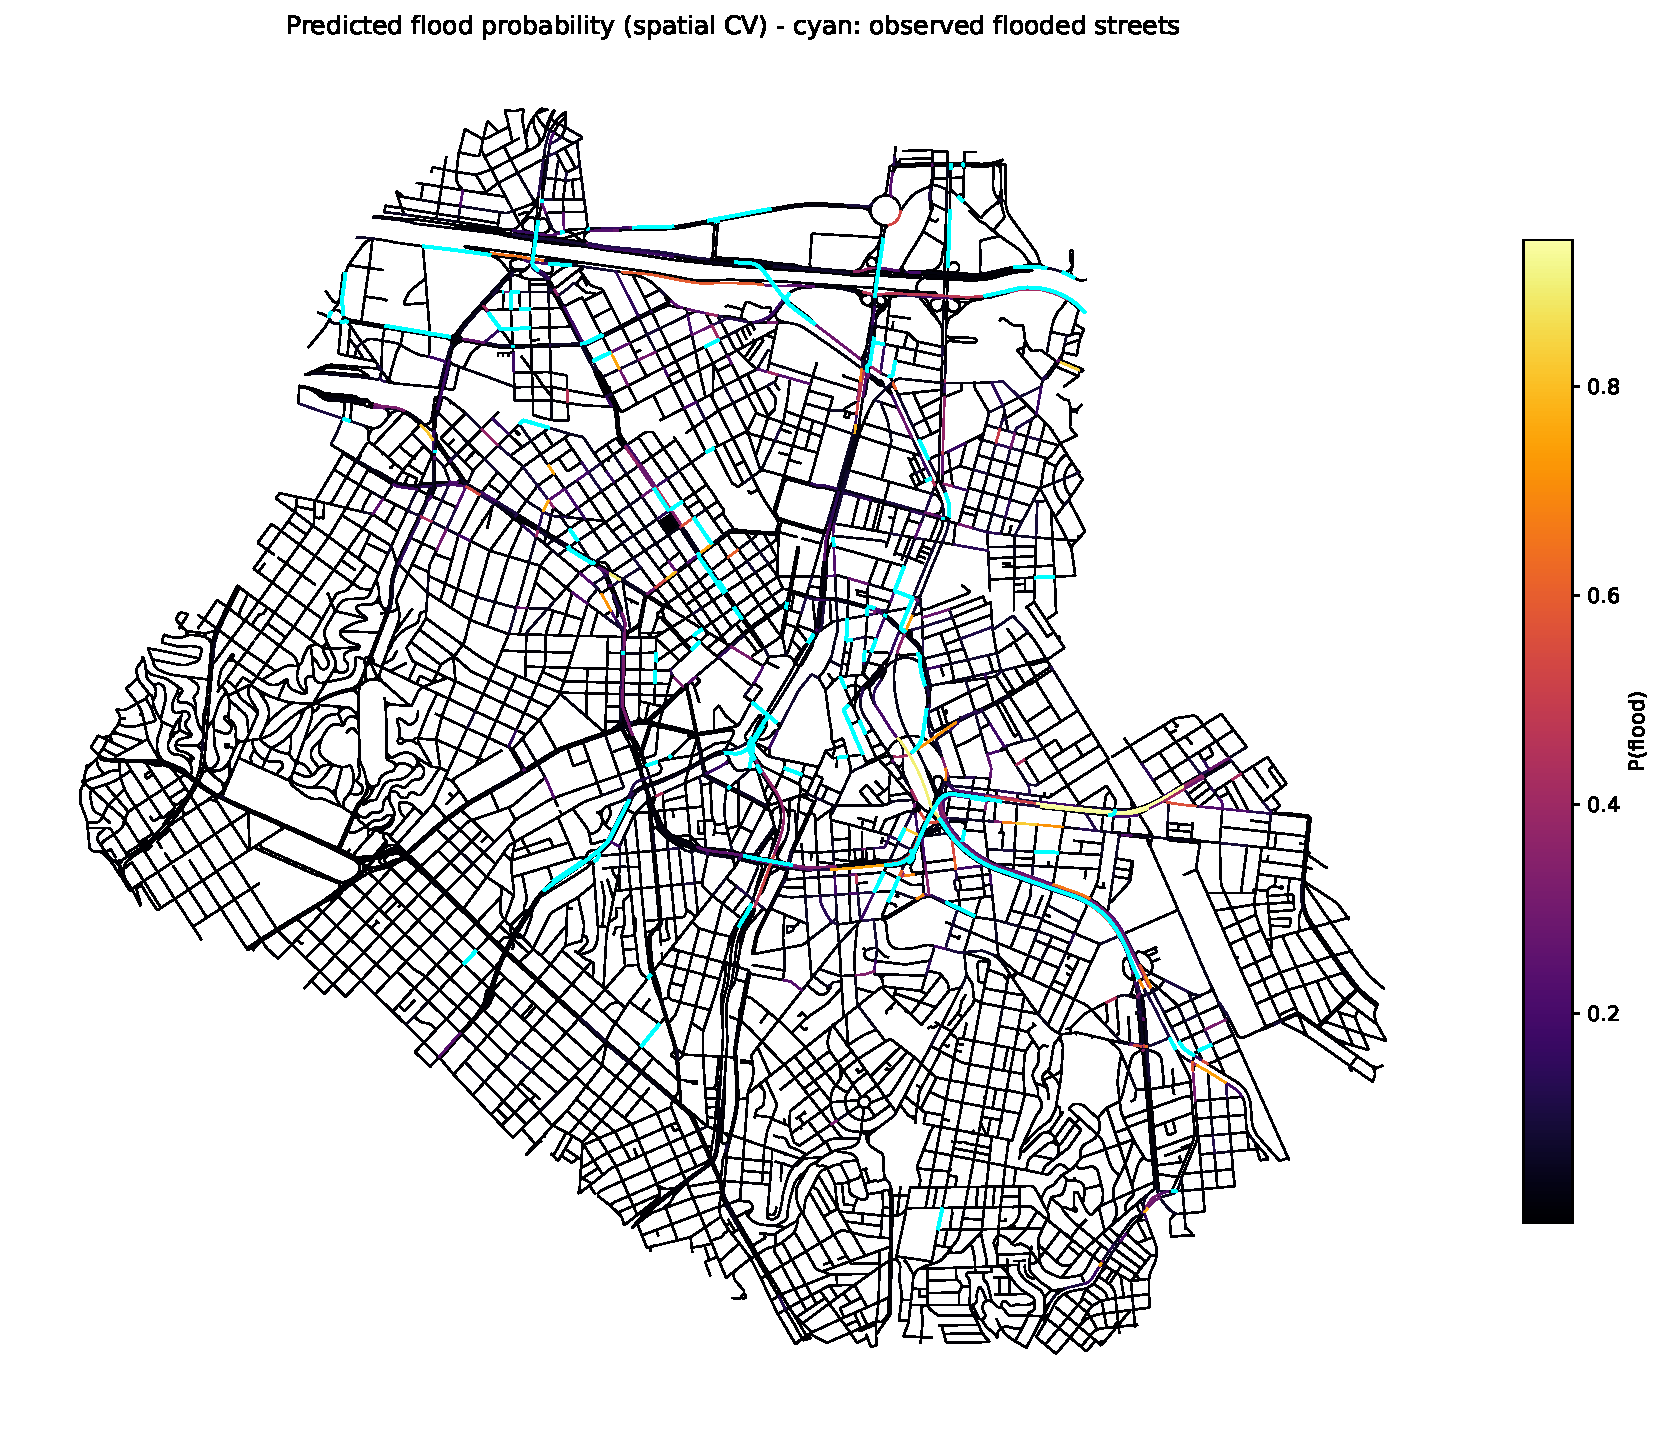
\includegraphics[width=0.85\columnwidth]{figures/flood_probability_map.pdf}
    \caption{Predicted flood probability under spatial cross-validation (each district predicted by a model that never saw it); cyan: observed flooded streets.}
    \label{fig:probmap}
\end{figure}

The signature is also robust in time. The contrast between flooded and non-flooded streets holds in the rainy season (December to March, 108 flooded streets) and in the dry season (47 flooded streets; the closeness effect is even larger, $r = 0.46$ against $0.25$), and the duration-weighted view (correlating the metrics with the total flooded hours per street) agrees with the binary one. Figure \ref{fig:monthly} shows the seasonality of the events.

\begin{figure}[H]
    \centering
    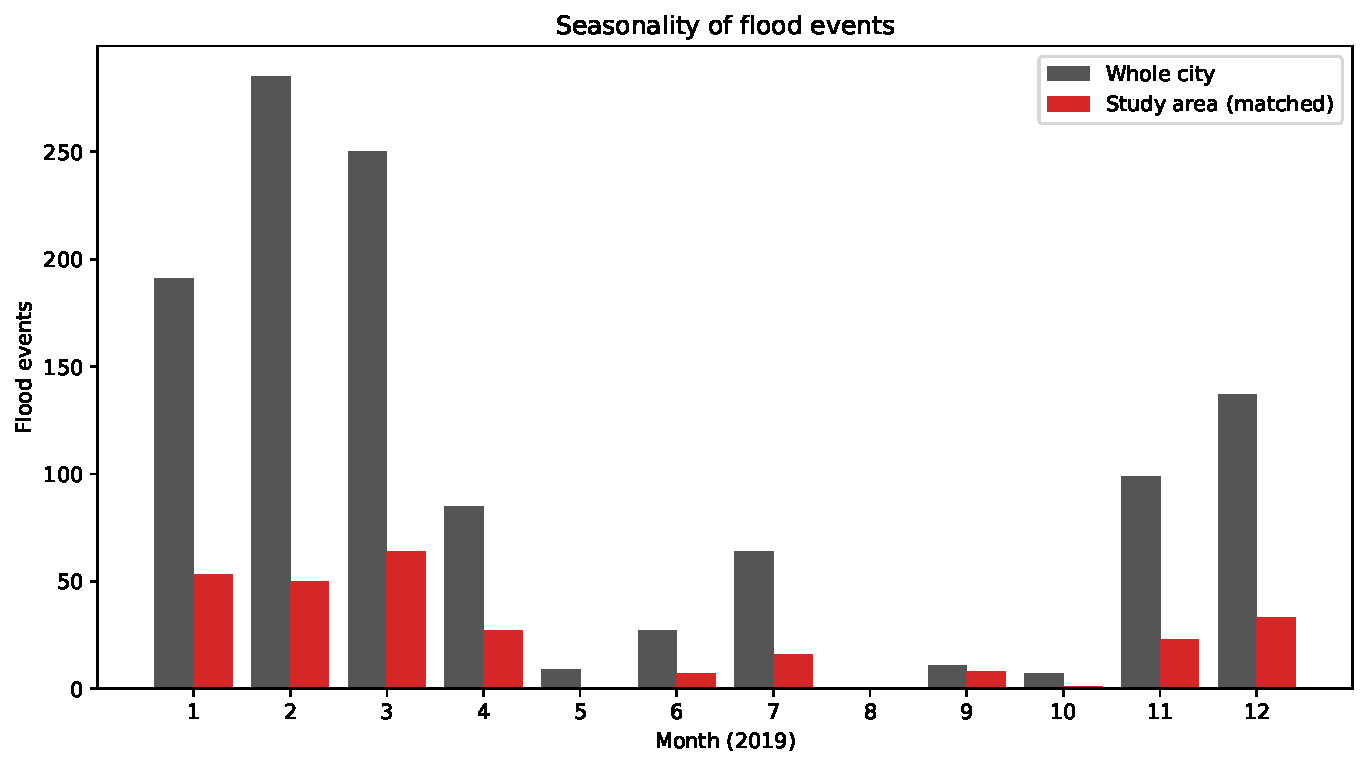
\includegraphics[width=0.75\columnwidth]{figures/monthly_events.pdf}
    \caption{Seasonality of the 2019 flood events, whole city and study area.}
    \label{fig:monthly}
\end{figure}

\section{Conclusion}\label{sec13}
\label{ch:conclusions}

Our analyses consist of investigating topological differences between flooded and non-flooded streets using graph theory and statistics, now at the scale of the whole city of São Paulo. We compare distributions of network metrics such as the mean shortest path, closeness, betweenness, degree, and vulnerability, control for terrain and street attributes, and verify the generalization district by district.

Upon analyzing both data sets of flooded and non-flooded streets, a clear signature emerges: the central streets flood more. The mean shortest path and closeness point toward streets located in close proximity to all others being more susceptible to flooding. The district decomposition is what makes this claim strong: the pattern is not a particularity of the center of São Paulo, it repeats area after area -- the betweenness effect is positive within every one of the 42 testable districts, and the median flooded street is more central than 75\% of the streets of its own district. And this is a huge problem, because those are the streets the city can least afford to lose: the vulnerability presents the largest topological effect, and the resilience simulation confirms independently that removing the flooded streets degrades the network more than a targeted attack of the same size.

It is crucial to note that the elevation is the strongest single factor -- floods are, first, a phenomenon of the low streets. The relevant finding is that part of the topological signature survives controlling for it: closeness, mean shortest path, and degree remain significant after accounting for elevation, slope, and street attributes. The betweenness tells a complementary story: it loses significance under the controls, but it is the most consistent metric across the city, positive within every one of the 42 testable districts. Consistency and independence from confounders are different claims, and the data supports each for different metrics.

Being central for the district and being central for the city are different roles, and the flooded streets are central in both readings; part of them are city-scale through-corridors, whose flooding is a problem for the whole city and not only for the district they cross. The strength of the within-district effect varies across the city in a way that no observable district characteristic (terrain relief, street-grid character, distance to the main rivers, size) explains, pointing again to the local drainage infrastructure as the missing variable.

It is crucial to note that we are observing a correlation, not establishing causation. However, these metrics reveal that the streets with the highest number of floods also have the greatest potential impact from a complex network perspective.

Floods occur due to several physical factors that impede proper drainage. Our terrain control relies on a 30 m elevation model, which is coarse relative to the micro-topography that governs drainage, and the arterial avenues of São Paulo were historically built over canalized streams (\textit{avenidas de fundo de vale}); a residual confounding by the buried hydrography cannot be excluded. Testing the signature against a high-resolution terrain model and the distance to the drainage network is the natural next step.

In future research, we also propose a transition from a point-based to a polygon-based representation of flood phenomena, given that flooding is inherently a spatially expansive event with the capability to render multiple streets inaccessible concurrently, and the extension of the analysis to multiple years. This proposed modification is anticipated to provide a more realistic and informative portrayal of flood dynamics.

One sentence summarizes this work: in every one of the 42 districts we could test, the streets that flood are the structurally important ones -- and removing them hurts the network more than a targeted attack of the same size.
\\

\newpage
\thispagestyle{empty}

\noindent \textbf{Availability of data and material:} The data that support the findings of this study are openly available at
\begin{verbatim}
    https://github.com/gioguarnieri/floods_in_sao_paulo
\end{verbatim}
The repository includes the executed notebooks (\texttt{Flood\_analysis\_OSMNX.ipynb}, \texttt{Flood\_analysis\_statistics\_OSM.ipynb}, \texttt{Flood\_analysis\_districts.ipynb}), the vulnerability computation (\texttt{compute\_vulnerability.py}), and the derived datasets.\\
\noindent \textbf{Funding}: This research was funded by the projects 446053/2023-6 and 140196/2022-6 from Conselho Nacional de Desenvolvimento Científico e Tecnológico (CNPq) and Conselho Nacional de Desenvolvimento Científico e Tecnológico PRINT project 88887.900891/2023-00.\\
\noindent \textbf{Competing interests:} The authors have no conflicts to disclose.\\
\noindent \textbf{Authors' contributions:} All authors contributed to the text and conceptualization. Soares did the computational work. Tomás made the plots.\\
\noindent \textbf{Acknowledgements}: Not applicable.


%% New references needed in sn-bibliography.bib (keys used above):
%%   boeing2017      - Boeing, G. (2017). OSMnx: New methods for acquiring, constructing, analyzing,
%%                     and visualizing complex street networks. Comput. Environ. Urban Syst. 65.
%%   page1999        - Page, L., Brin, S., Motwani, R., Winograd, T. (1999). The PageRank citation
%%                     ranking: Bringing order to the web. Stanford InfoLab.
%%   benjamini1995   - Benjamini, Y., Hochberg, Y. (1995). Controlling the false discovery rate. JRSS B 57(1).
%%   dersimonian1986 - DerSimonian, R., Laird, N. (1986). Meta-analysis in clinical trials. Control. Clin. Trials 7(3).
%%   gil2017         - Gil, J. (2017). Street network analysis "edge effects": Examining the sensitivity
%%                     of centrality measures to boundary conditions. EPB 44(5).

\bibliographystyle{sn-nature}
\bibliography{sn-bibliography}% common bib file


\end{document}
